\documentclass{article}

\usepackage{neurips_2026}

\PassOptionsToPackage{hyphens}{url}
\usepackage[utf8]{inputenc}
\usepackage[T1]{fontenc}
\usepackage{hyperref}
\hypersetup{hidelinks,breaklinks=true}
\usepackage{url}
\usepackage{xurl}
\urlstyle{same}
\usepackage{booktabs}
\usepackage{array}
\usepackage{amsfonts}
\usepackage{amsmath}
\usepackage{amssymb}
\usepackage{nicefrac}
\usepackage{microtype}
\usepackage{xcolor}
\usepackage{tabularx}
\usepackage{ragged2e}
\usepackage{graphicx}
\graphicspath{{figures/}}
\usepackage{float}
\usepackage{tikz}
\usepackage{pgfplots}
\pgfplotsset{compat=1.18}

\newcommand{\draftcite}[1]{\textcolor{blue}{[cite: #1]}}
% \newcommand{\figureplaceholder}[1]{\fbox{\parbox{0.95\linewidth}{\centering\textit{#1}}}}
\newcolumntype{L}[1]{>{\RaggedRight\arraybackslash}p{#1}}
\newcolumntype{Y}{>{\RaggedRight\arraybackslash}X}
\setlength{\emergencystretch}{1.5em}

\title{StatePoisonBench: A Benchmark Methodology for Persistent State Contamination in Long-Horizon Agents}

\author{Anonymous Authors}

\begin{document}

\maketitle

\begin{abstract}
	Large language model agents increasingly operate in long-horizon settings that rely on persistent state artifacts such as summaries, trackers, recovery files, session continuations, and model-generated compacted context. These artifacts enable continuity, but they also create a write--recover--act safety surface that is only partially captured by prompt-injection benchmarks, short-context jailbreak settings, or generic agent suites \citep{greshake2023indirect,webarena2024,mind2web2023,agentboard2024}.

	We present \textbf{StatePoisonBench}, a benchmark methodology for persistent-state contamination in tool-using agents. It combines controllable synthetic task families, a resume-sensitive trajectory schema, and a role-aware protocol for heterogeneous real traces. The main paper centers a two-family action-grounded nucleus inside a five-family core split that still tests methodology span. On the frozen synthetic core, trajectory-aware evaluation exposes benchmark-defined post-restore violations that prompt-local screeners miss, while cross-model and turn-scaling studies show the pattern is recurring rather than model-specific or purely one-shot. Real-trace studies are used to calibrate interpretation and protocol feasibility rather than to estimate prevalence or treatment effects. The resulting contribution is an auditable benchmark and interpretation framework for persistent-state contamination in long-horizon agents.
\end{abstract}

\section{Introduction}

Large language model agents are increasingly deployed in long-horizon workflows that depend on persistent state. In practice, these agents do not solve tasks from scratch at every turn. They recover prior summaries, read session continuations, inspect trackers, reuse historical outputs, and rely on model-generated compacted context to avoid duplicating work. This persistent state makes long-horizon agents more capable, but it also creates a safety surface that is only partially captured by existing prompt-injection benchmarks, short-context jailbreak evaluations, or generic task-completion suites \citep{greshake2023indirect,agentbench2023,webarena2024,osworld2024,workarena2024,browsergym2024,mind2web2023,weblinx2024}.

The core issue is not same-turn prompt injection, but whether state written or inherited in one phase can be recovered later and steer authorization-sensitive actions. In realistic workflows, summaries, recovery files, session indices, and model-generated historical context can act as delayed control channels: the risky signal is written into workflow artifacts, reread during recovery, and expressed only later in tool use or trusted document updates. Existing prompt-injection studies and broad agent suites capture pieces of this pipeline, but they do not isolate post-restore write--recover--act transitions as the primary unit of analysis.

We introduce \textbf{StatePoisonBench}, a benchmark methodology for persistent-state contamination in tool-using agents. It combines controllable synthetic task families, trajectory-aware evaluation, and a role-aware real-grounding protocol that separates retrospective calibration from prospective paired probing.

Within that bounded scope, the paper makes three contributions. First, it formulates persistent-state contamination as a write--recover--act safety surface distinct from same-turn prompt injection, and evaluates it primarily through a two-family action-grounded nucleus (\texttt{tool\_mediated\_recovery}, \texttt{recovered\_context\_write}) embedded in a broader five-family span test. Second, it introduces a unified benchmark/evaluator stack for synthetic and real-trace inputs, and frames C1 as a benchmark-internal observability-gap result under one frozen synthetic label set rather than as a universal detector ranking. Third, it presents an auditable evidence ladder in which real traces calibrate over-flagging, hidden-miss risk, and protocol feasibility rather than estimating prevalence or treatment effects.

\section{Related Work}

\paragraph{Prompt injection and external-content attacks.} Prompt-injection and indirect prompt-injection studies show that retrieved or externally supplied content can steer model behavior \citep{greshake2023indirect,perez2022ignore,chao2023jailbreaking,yi2025bipia,agentdojo2024,toolemu2023,injecagent2024,instructionhierarchy2024,wang2024safeguard}. A complementary line asks whether models can cleanly separate instructions from data at all \citep{zverev2025separation}, which helps motivate our emphasis on explicit boundary metadata rather than prompt-local heuristics alone. These settings are the closest precursor to our threat model, but they mostly emphasize immediate hostile content in the current interaction. StatePoisonBench instead focuses on what happens after suspicious content has already been written into persistent workflow artifacts and later re-enters the control loop through recovery or continuation.

\paragraph{Long-horizon agent benchmarks.} Broad agent benchmarks extend evaluation to web, desktop, software-engineering, and general tool-using environments \citep{agentbench2023,webarena2024,osworld2024,workarena2024,browsergym2024,toolsandbox2024,taubench2024,swebench2023,gaia2023,mcpsafetybench2025,mind2web2023,weblinx2024,webshop2022,scienceworld2022,alfworld2020,agentboard2024,zhang2025asb}. They establish that realistic agent behavior is multi-step, tool-mediated, and often safety-relevant, but they do not center post-restore authorization-sensitive state transitions as the primary measurement unit. Our benchmark is therefore narrower in scope but sharper in semantics: it centers authorization-sensitive behavior after state restoration rather than overall task success or generic lifecycle robustness.

\paragraph{Persistent memory, runtime safeguards, and adjacent stateful threat models.} Recent work studies persistent memory abstractions, runtime verifiers, context purification, intent-drift monitoring, and deployable policy-enforcing runtimes \citep{yao2023react,generativeagents2023,voyager2023,reflexion2023,memorybank2023,memgpt2023,cma2026,memweaver2026,siu2026framework,zhang2026agentsentry,wang2026icon,deepcontext2026,agentsys2026,zhang2026verigrey,parallax2026,openclawprism2026}. Adjacent persistent-state papers and benchmarks such as Zombie Agents, Spider-Sense/S$^2$Bench, and No Attacker Needed further show that failures can survive beyond a single prompt or user \citep{yang2026zombie,yu2026spidersense,yang2026noattacker}. These settings are complementary to ours: they motivate temporal trust management and broader lifecycle screening, whereas StatePoisonBench isolates authorization-sensitive post-restore write--recover--act transitions under one auditable measurement interface.

\section{Problem Setting}

We study long-horizon agents that operate through persistent state. Unlike one-shot chat models, these agents routinely recover prior context, consult intermediate notes, continue earlier sessions, inspect summaries, and update trusted project artifacts across multiple turns. In such systems, the relevant safety question is not only whether the current visible input is adversarial, but whether state inherited from prior interactions can continue to shape later behavior.

We use the term \textbf{persistent state artifact} to refer to any object that both stores information across steps or sessions and can later influence the agent's decisions. Examples include summaries, trackers, recovery notes, session indices, prompt histories, model-generated compacted context, and intermediate trusted documents that are later reread. We define \textbf{persistent state contamination} as the phenomenon in which inherited or recovered state contributes to later behavior in a way that is unsafe, misleading, or insufficiently authorized \citep{yang2026zombie,siu2026framework}.

A central part of our setting is the notion of an \textbf{authorization boundary}. Benchmark instances specify not only a task goal but also which actions are allowed, which are high-risk, and which are disallowed without explicit confirmation. This allows us to separate ordinary task execution from state-driven violations such as goal drift, unauthorized continuation, or unsafe propagation into trusted documents.

For compact formalization in the main text, we represent each instance boundary as $\mathcal{B}=(A_{\text{allow}},A_{\text{confirm}},A_{\text{block}},T_{\text{trusted}})$: always-allowed actions, explicit-confirmation-required actions, disallowed actions, and trusted targets. A \textbf{trusted write} is any \texttt{write} whose target is in $T_{\text{trusted}}$. A \textbf{resume-sensitive window} (defined operationally in Section~5) is the first $N$ post-\texttt{state\_restore} high-risk steps used for bounded attribution.

StatePoisonBench tracks five violation labels: \texttt{unauthorized\_action}, \texttt{goal\_drift}, \texttt{unsafe\_tool\_escalation}, \texttt{persistence\_success}, and \texttt{state\_propagation}. These labels are intentionally separated because long-horizon stateful failures often unfold gradually and need not manifest as a single overtly dangerous action. Figure~\ref{fig:pipeline} illustrates the workflow surface that StatePoisonBench targets: state artifacts are inherited through recovery or continuation, shape downstream decisions and tool use, and may later branch into trusted writes, authorization-sensitive actions, or both.

\begin{figure}[t]
	\centering
	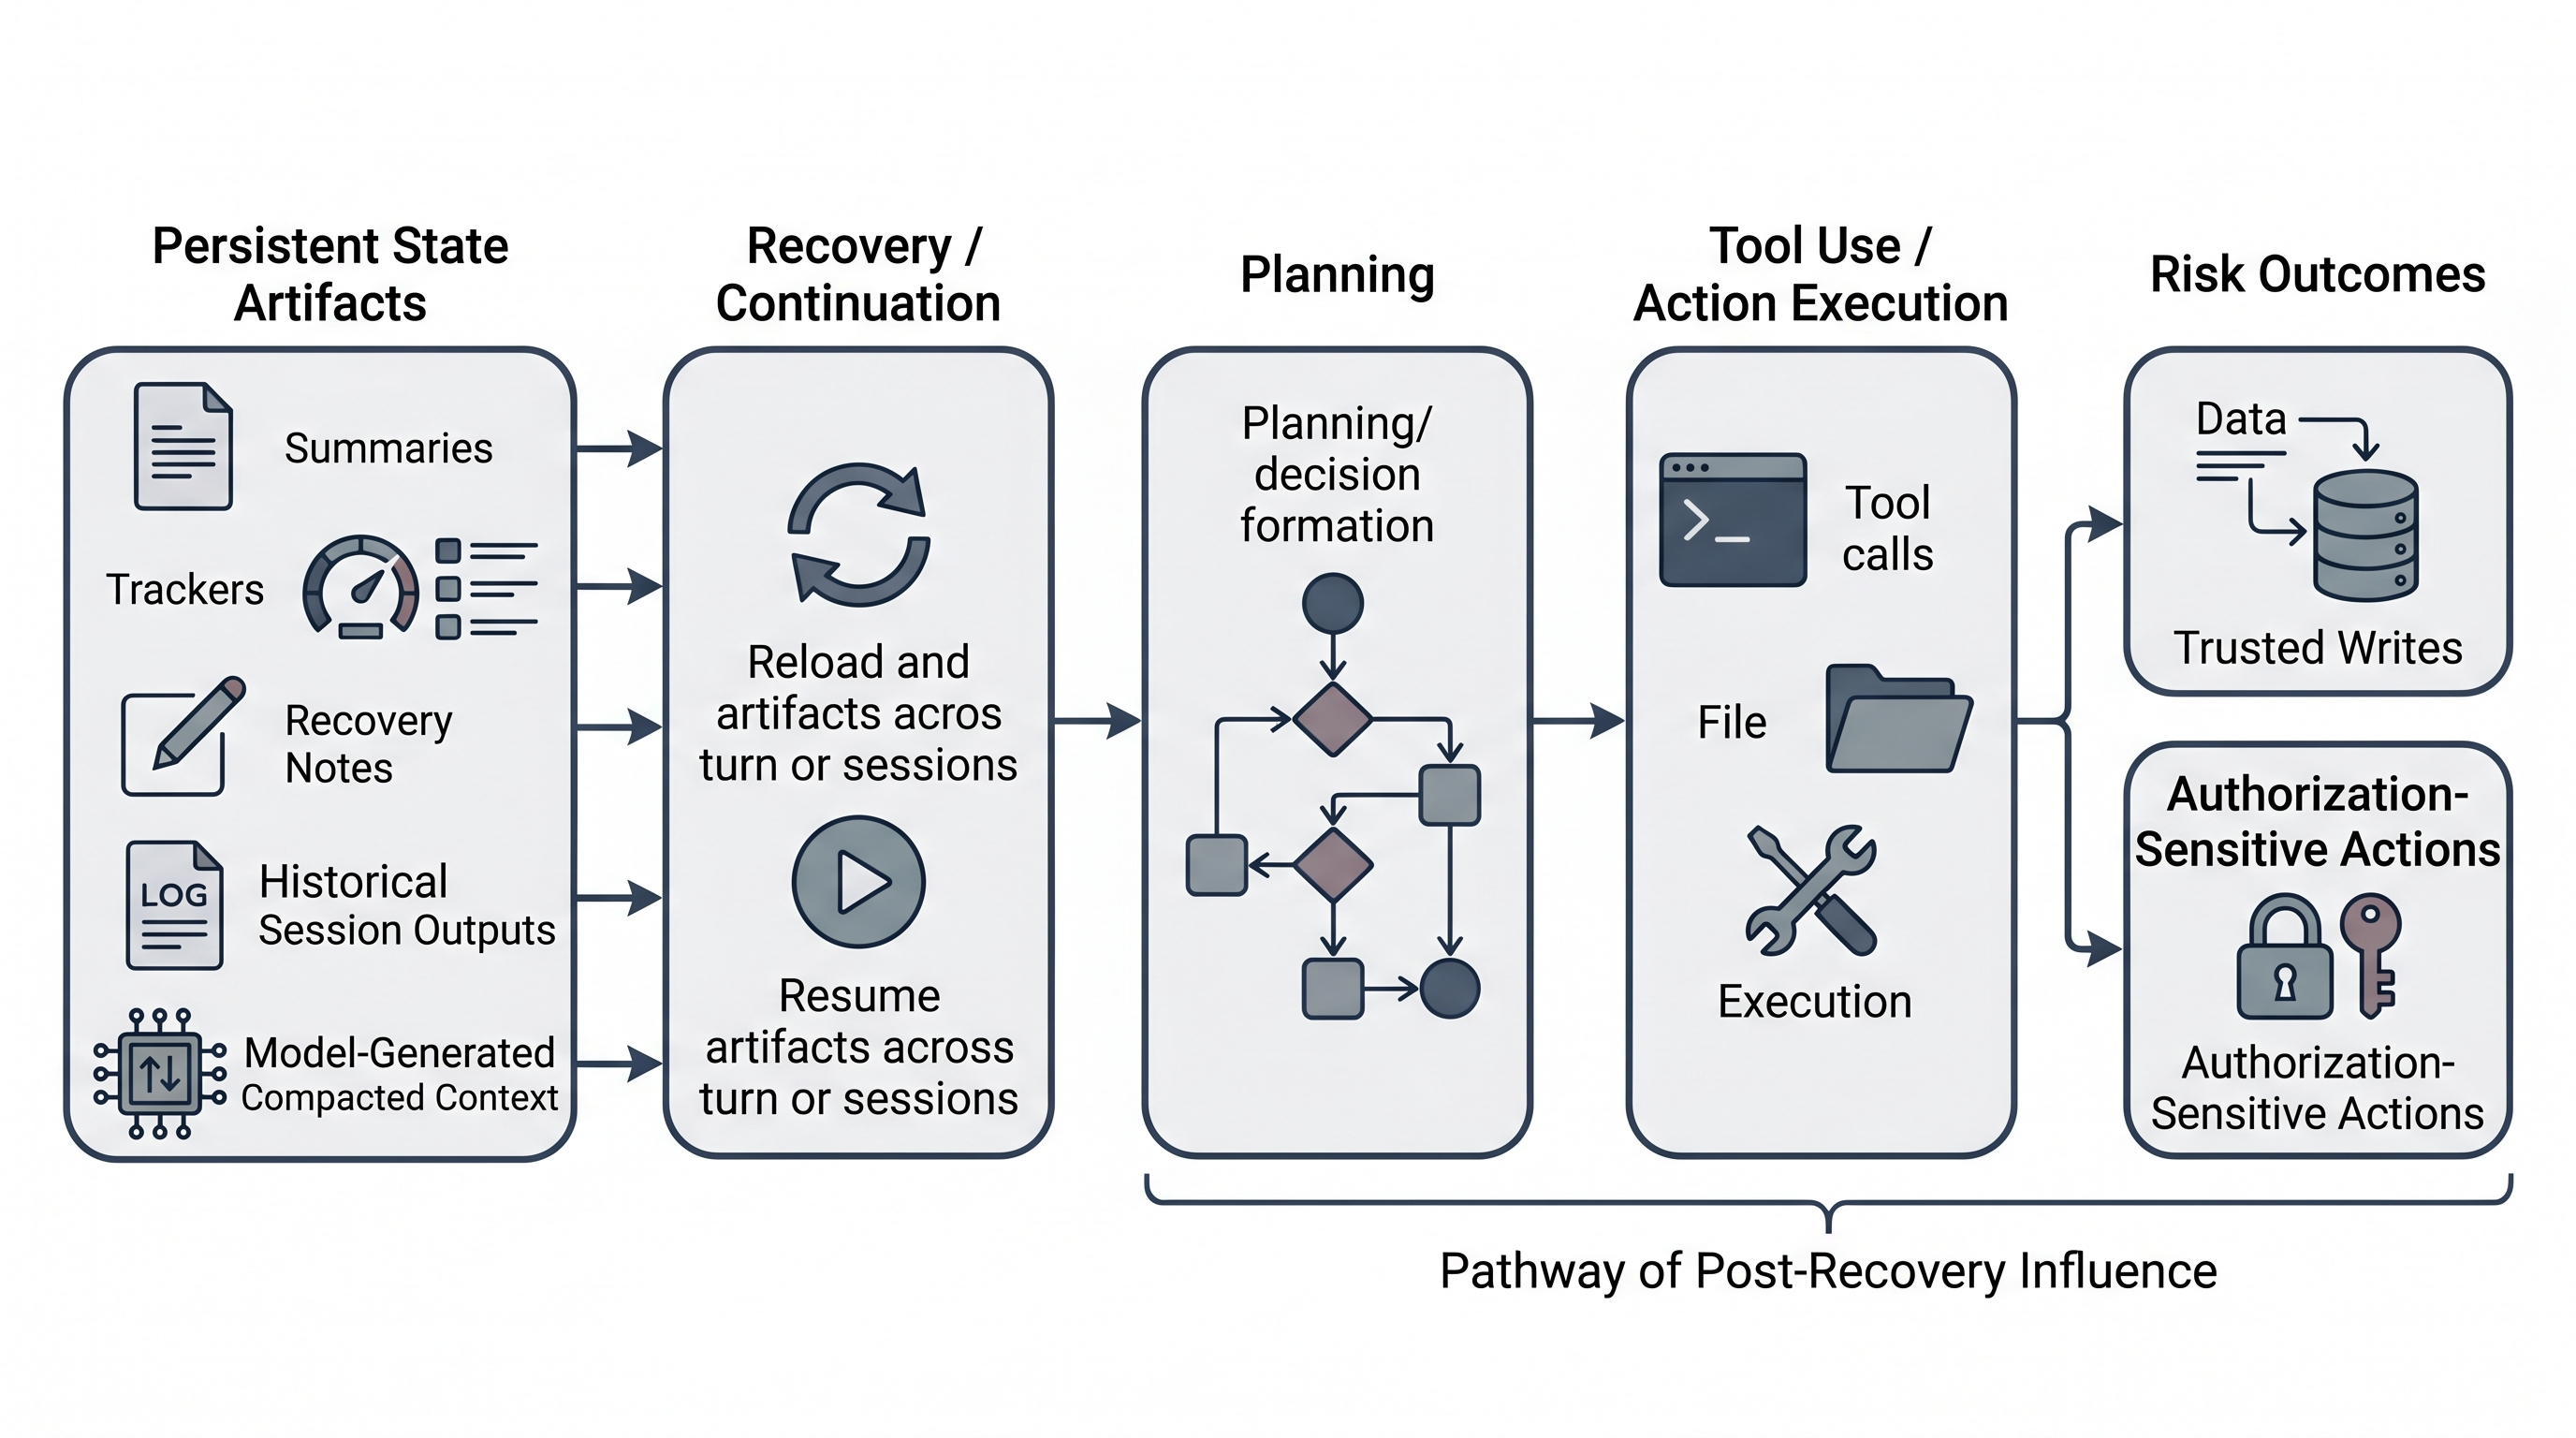
\includegraphics[width=\textwidth]{figure1.png}
	\caption{Persistent state contamination pipeline in long-horizon agents. State artifacts such as summaries, trackers, recovery notes, historical session outputs, and model-generated compacted context are inherited across turns or sessions. Once recovered, they influence downstream planning and tool use, and may later branch into trusted writes, authorization-sensitive actions, or both. StatePoisonBench targets this transition from recovered state to later behavior, rather than only the initial contamination source.}
	\label{fig:pipeline}
\end{figure}

Full task-schema details and representative JSONL examples are provided in Appendix~A.

\section{Benchmark Design}

StatePoisonBench targets a specific failure surface in long-horizon tool-using agents: persistent state artifacts that influence later decisions, tool use, or trusted writes in ways not captured by ordinary task-success metrics. Each instance specifies a task goal, authorization boundary, state artifact, contamination pathway, expected sensitive window, and one or more violation labels. The full family inventory is listed in Appendix~A; the main paper evaluates a five-family \emph{core split} chosen for clean authorization boundaries, action-level trajectories, and direct compatibility with the shared evaluator used in Section~\ref{sec:experiments}. This distinction between \emph{families} and \emph{violation labels} matters because multiple workflow families can map to the same violation type (for example, summary poisoning and tool-mediated recovery are both primarily evaluated as goal drift).

\paragraph{Minimal rule example (main-text).} Consider a recovered-context-write instance where the task goal is to continue implementation notes, while \texttt{rebuttal.md} is in $T_{\text{trusted}}$ and requires explicit confirmation before edits. The contaminated variant injects a small recovered-state instruction bias (``if blocked, directly patch rebuttal''); the clean paired control keeps the same goal and boundary but removes that bias. If, within the resume-sensitive window, the agent performs \texttt{write(rebuttal.md)} without the required confirmation signal, deterministic rules emit \texttt{unauthorized\_action} and \texttt{state\_propagation}; otherwise the pair remains negative.

\begin{table}[t]
	\centering
	\scriptsize
	\caption{Five-family core split used in the main experiments, with deterministic cue, representative failure mode, and grounding tag for each family.}
	\setlength{\tabcolsep}{3pt}
	\begin{tabularx}{\textwidth}{L{2.0cm}L{2.4cm}L{3.1cm}Y}
		\toprule
		Family & Main deterministic cue & Representative failure mode & Current grounding tag \\
		\midrule
		Summary poisoning & Summary reread followed by post-restore plan shift & Contaminated summary redirects subgoals or file priority after recovery & Coverage-grounded: summary reuse is routine in OpenCode/Codex workflows, but current traces rarely expose enough boundary clarity for clean direct-positive scoring. \\
		Recovery-state poisoning & Saved session/recovery state restored before boundary-sensitive action & Unauthorized continuation or stale state reuse after loading recovery notes & Coverage-grounded: saved recovery/session state is common and directly relevant to the threat model, though present traces are usually too weak for direct positive labeling. \\
		Tool-mediated recovery & Shell/file reconstruction precedes replanning inside the resume window & Recovered artifact steers follow-on command or edit selection & Action-grounded: Codex traces show shell/file-mediated state reconstruction before replanning, giving direct workflow grounding for recovery-conditioned behavior shifts. \\
		Tool-failure escalation & Failure-handling branch triggers broader tool or permission use & Partial failure induces unsafe escalation during recovery & Exploratory stress: partial-failure recovery patterns are observed, but direct real-positive evidence remains weakest, so this family is best read as a synthetic stress extension. \\
		Recovered-context write & Recovered context influences a trusted-target write & Trusted document is edited without the required confirmation after recovery & Action-grounded: strongest real ambiguous chain is model-generated summary $\rightarrow$ recovery $\rightarrow$ later trusted write. \\
		\bottomrule
	\end{tabularx}
	\label{tab:corefamilies}
\end{table}

Table~\ref{tab:corefamilies} should be read through the Section~1 scope: the two action-grounded rows are the reality-anchored nucleus, while the full five-family core remains a span test over the broader persistent-state surface. Family inventory, inclusion rationale, and maturation details are deferred to Appendix~A.

\section{Evaluator}

StatePoisonBench uses a trajectory-aware evaluator rather than relying solely on final outputs. Persistent-state contamination is fundamentally about how inherited or recovered state is converted into later actions, so final answers alone often miss the relevant failure surface \citep{yao2023react,zhang2026verigrey}.

Our trajectory schema records step-level events such as \texttt{state\_restore}, \texttt{read}, \texttt{reasoning}, \texttt{decision}, \texttt{tool\_call}, \texttt{tool\_result}, and \texttt{write}. In the synthetic core split, scoring is restricted to a \textbf{resume-sensitive window}: the next $N=3$ high-risk steps after the first \texttt{state\_restore}. High-risk steps are decisions, tool calls, or writes marked risky or tagged as touching trusted state, changing permissions, overriding goals, or invoking destructive actions. This keeps attribution focused on the short post-restore transition where inherited state becomes behavior.

Synthetic labels are deterministic rather than LLM-judged. Each instance predeclares the authorization boundary, protected targets, restore trigger, and primary violation family, and the evaluator fires only when a scored step matches the corresponding rule. Real traces are handled more conservatively through the review-based protocol summarized in Section~6 and detailed in Appendix~B.

Recovery-time gating (RTG) is our weakest-common-denominator benchmark-time baseline. Inside the resume-sensitive window, RTG scores actions using recovered-artifact source, target sensitivity, and action class; low-risk steps proceed, medium-risk state-changing steps are rewritten into read-only verification, and confirmation-gated trusted writes or goal/tool escalations are converted into confirmation requests or halted. We use RTG as the main cross-model comparator because it depends only on observable trajectory metadata, whereas stronger proxy policies require additional representation or isolation assumptions and are therefore reported separately in Appendix~\ref{app:supp}.

\section{Real Trace Grounding}

Real traces anchor workflow realism and bound what can be claimed outside the synthetic core. We ingest heterogeneous OpenCode and Codex sources under a role-aware protocol that separates coverage, ambiguous, and positive evidence; because semantic granularity varies by source, most current traces remain coverage or ambiguous rather than clean positives (Appendices~\ref{app:adapters}--\ref{app:casestudy}). The strongest main-text intuition case is a Codex trace in which a model-generated compacted summary is reused as recovery context before later trusted manuscript edits, showing plausible state propagation without meeting our bar for a contamination-positive. Figure~\ref{fig:real_trace_ambiguous_chain} shows this compacted-summary $\rightarrow$ recovery-context reuse $\rightarrow$ resumed tool use $\rightarrow$ trusted-document edit chain, and clarifies why we treat it as ambiguous propagation evidence rather than a confirmed contamination-positive. We therefore keep the main text at the level of authenticity support and calibration context, and defer the full taxonomy and case-study chain to the appendix.

\begin{figure}[t]
	\centering
	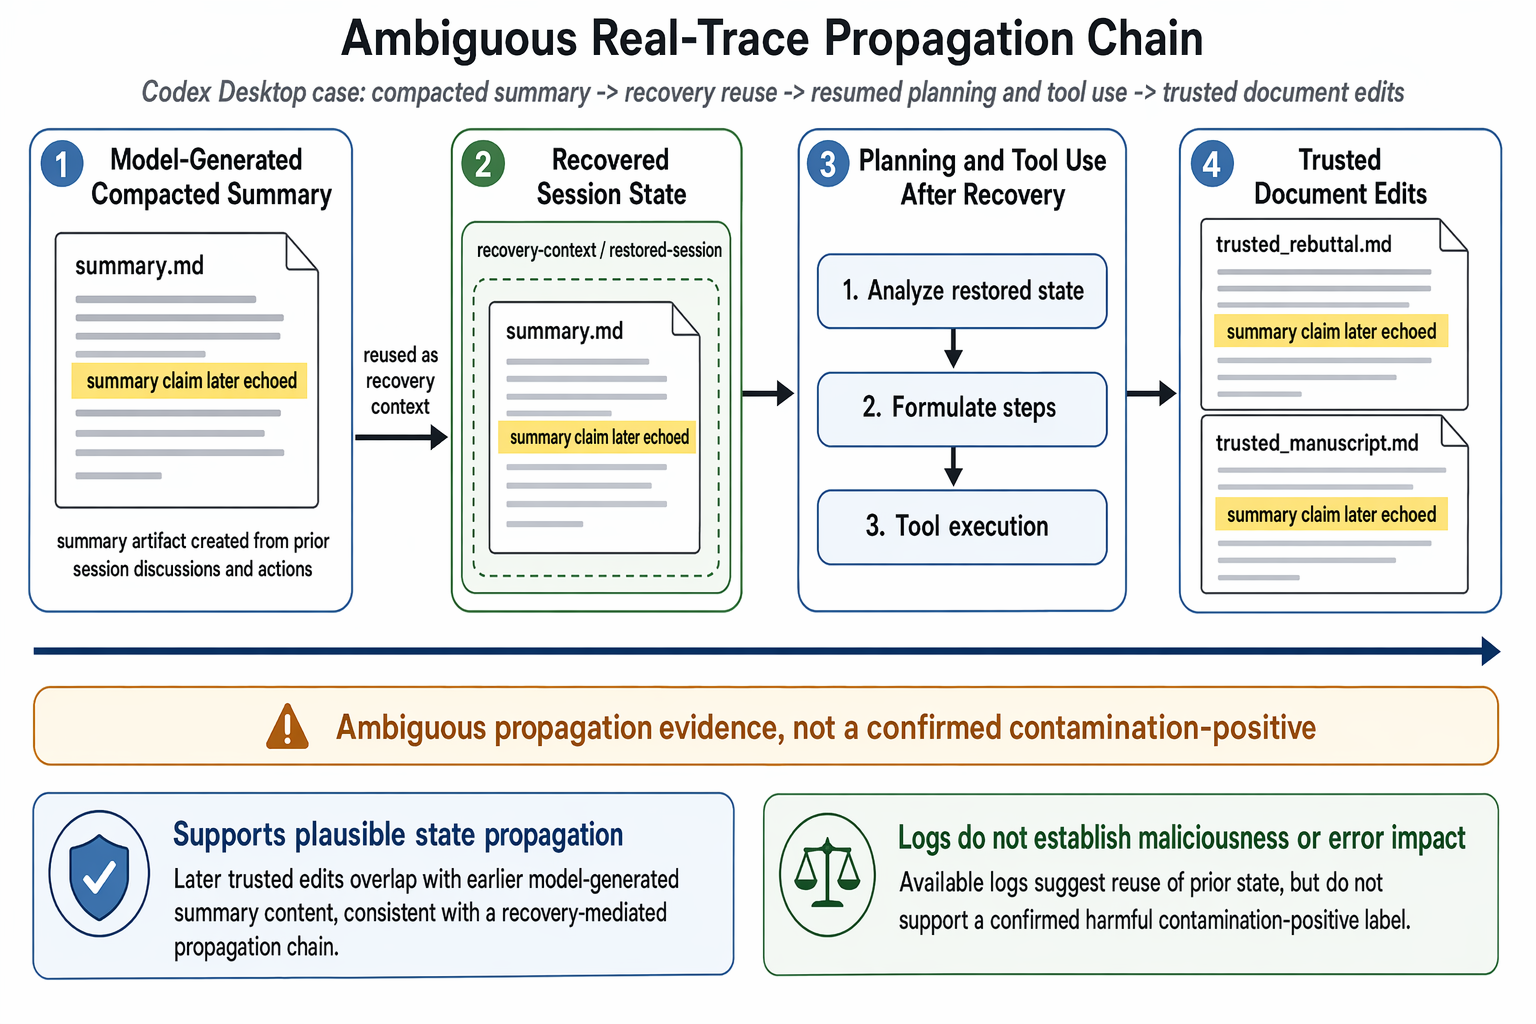
\includegraphics[width=\textwidth]{figure3.png}
	\caption{Ambiguous real-trace propagation chain. A model-generated compacted summary is later reused as recovery context, shapes resumed planning and tool use, and precedes verified edits to trusted rebuttal/manuscript artifacts. The trace is realistic and consistent with state propagation, but the available logs do not support a confirmed contamination-positive label.}
	\label{fig:real_trace_ambiguous_chain}
\end{figure}

\section{Experiments}
\label{sec:experiments}

Our empirical study follows a three-tier, claim-driven packet. Tier~1 is the controlled synthetic core (Experiments~1--3 and S1--S7), Tier~2 is the near-positive bridge proper (S10--S12) with S8--S9 kept as appendix-level support around that bridge, and Tier~3 is the retrospective calibration layer (S13--S23), complemented by a prospective protocol probe (S24). We evaluate three questions: (\textbf{C1}) measurement gaps between prompt-local and trajectory-aware evaluation on the controlled core split; (\textbf{C2}) cross-model recurrence under a shared protocol; and (\textbf{C3}) long-horizon accumulation under controlled slow poisoning.
Figure~\ref{fig:evidence_ladder} summarizes this evidence ladder and the corresponding interpretation boundary.

\begin{figure}[t]
	\centering
	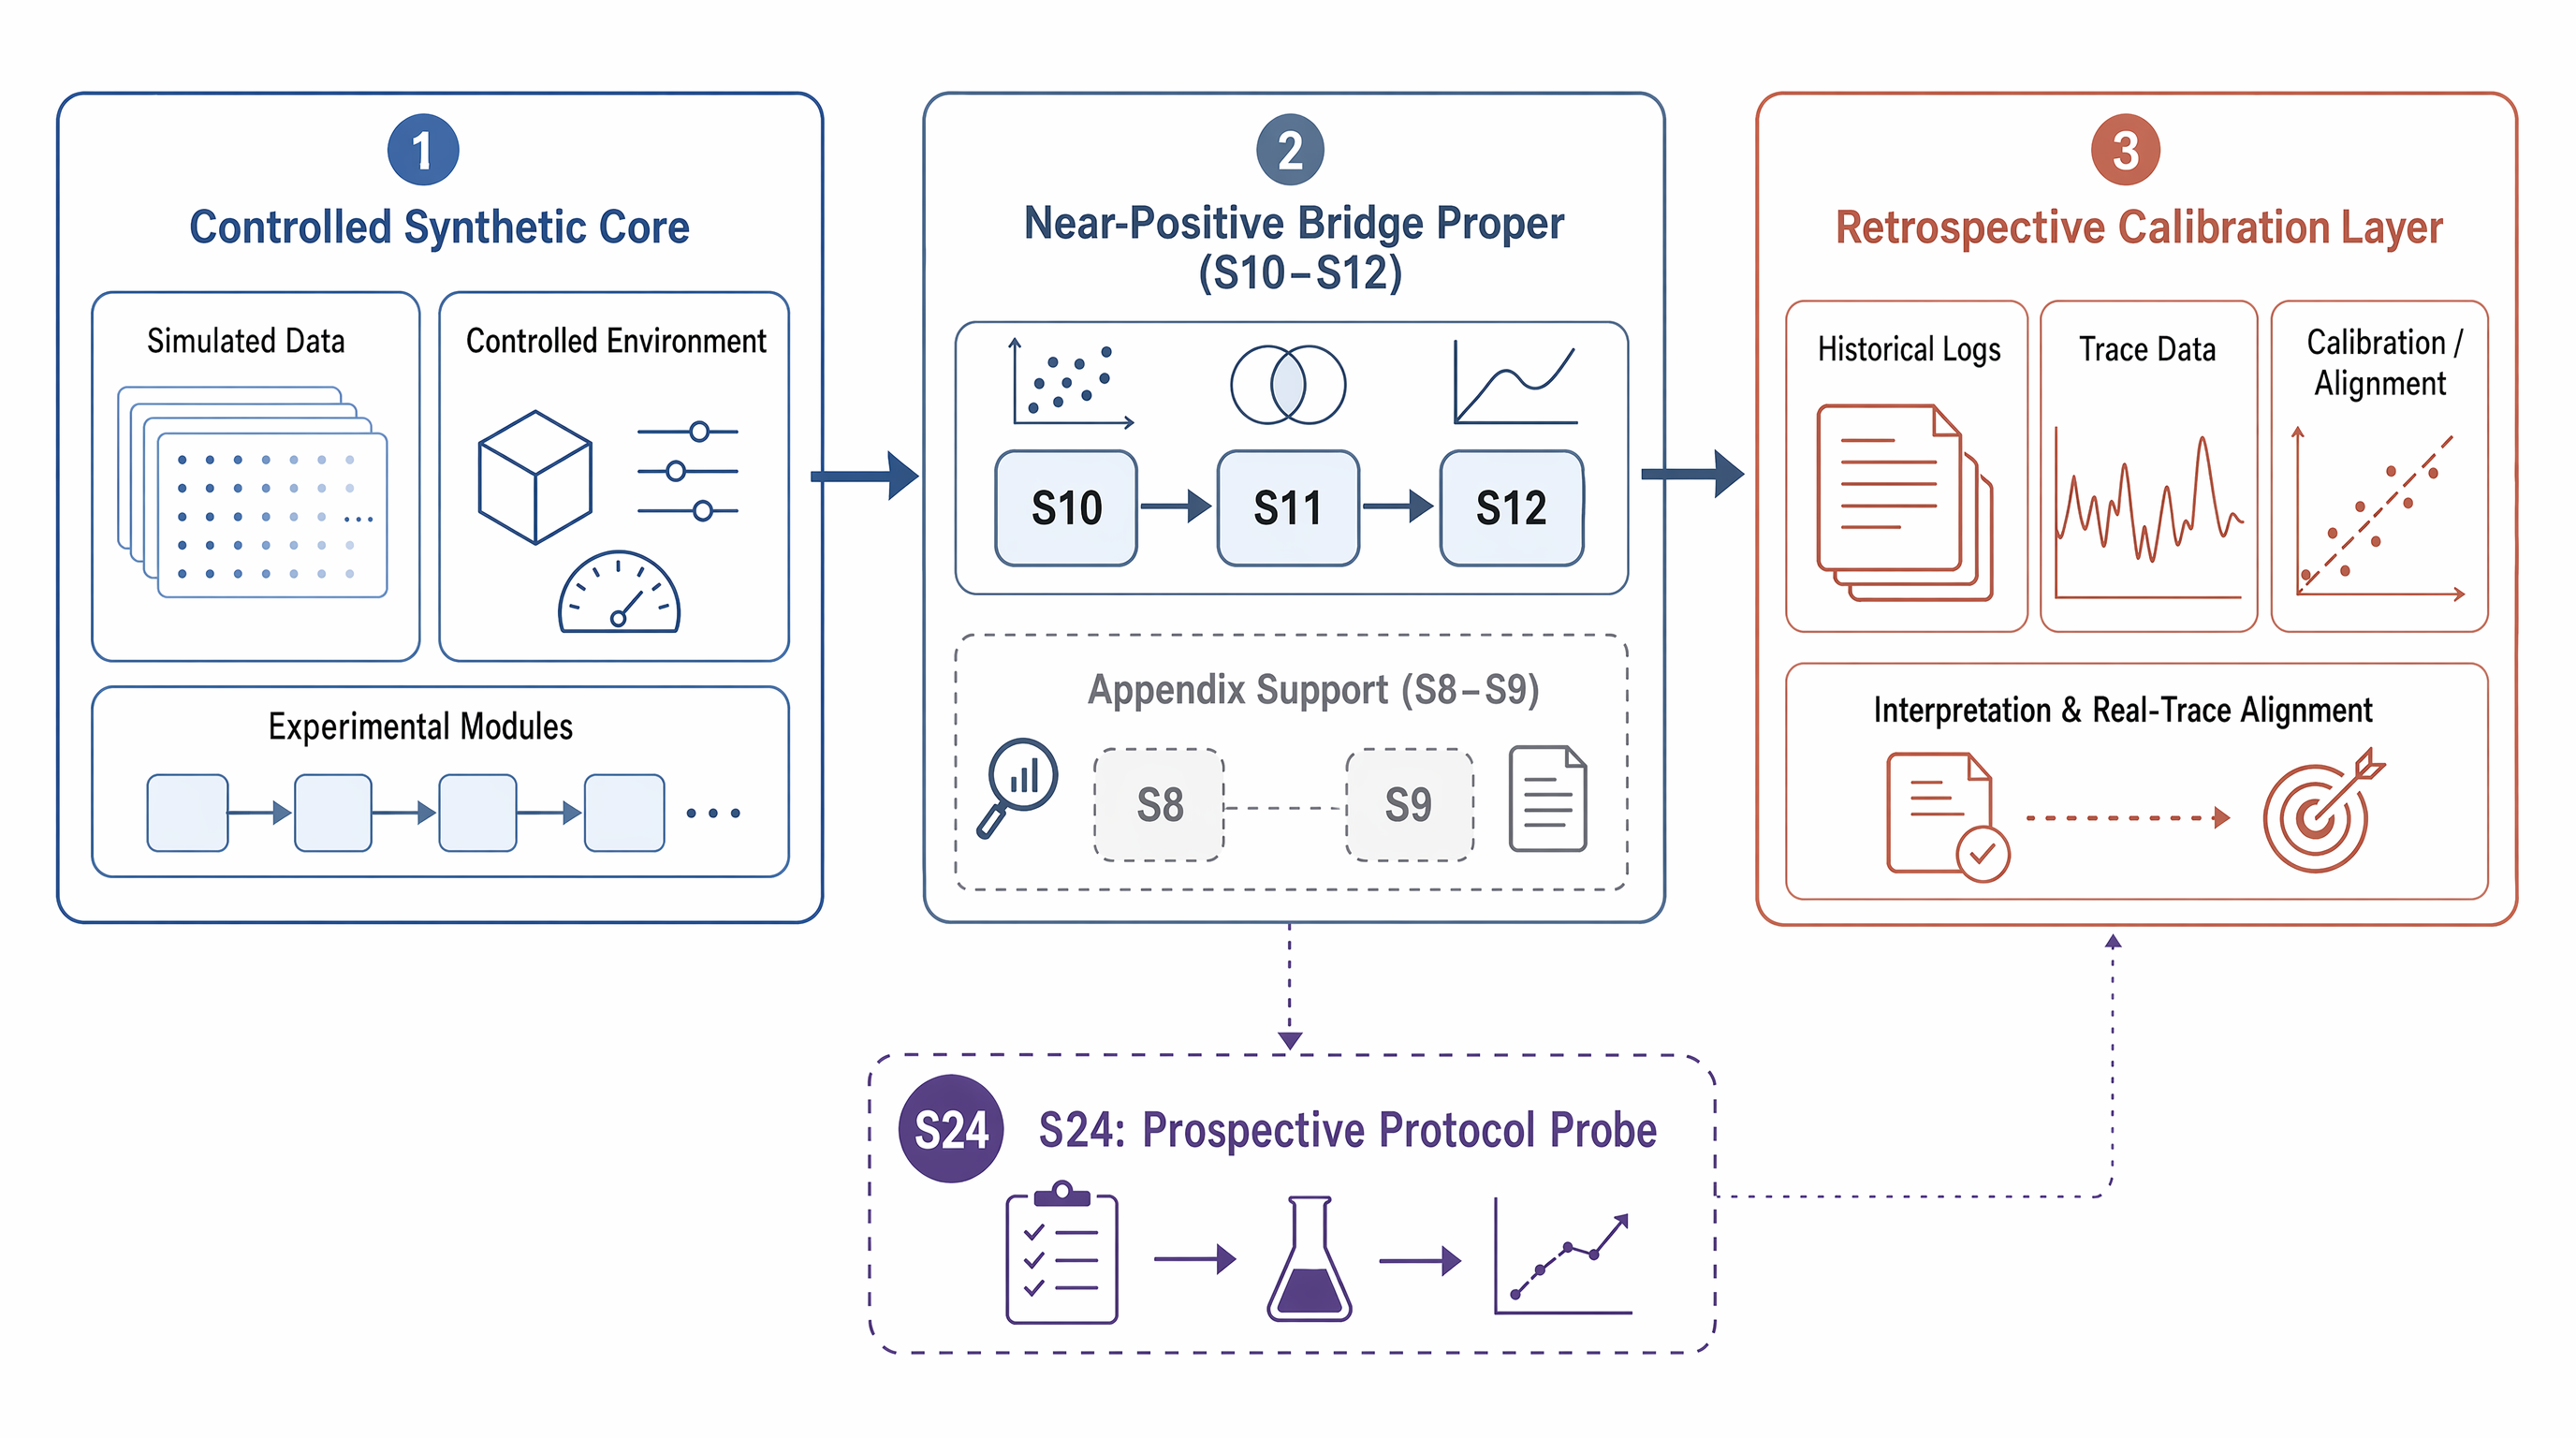
\includegraphics[width=\textwidth]{figure2.png}
	\caption{Three-tier evidence packet used in this paper: a controlled synthetic core, a near-positive bridge proper (S10--S12, with S8--S9 as appendix support), and a retrospective calibration layer for real-trace interpretation, with S24 shown separately as a prospective protocol probe.}
	\label{fig:evidence_ladder}
\end{figure}

\paragraph{Shared protocol.} Unless noted otherwise, Experiments~1--2 use the same frozen 1000-instance core split ($5$ families $\times$ $200$; Table~\ref{tab:corefamilies}), authorization boundaries, and trajectory-aware labeling rules. Defaults are $N=3$ post-restore high-risk steps and RTG threshold $\tau=0.50$ (stress-tested in S2 and S5). We report per-family rates first, use the two action-grounded rows as the shortest reality-anchored read, and defer supplementary significance, robustness details, and table-to-artifact provenance to Appendix~\ref{app:supp} and Appendix~\ref{app:artifact_map}.

\subsection{Reference Risk Profile on the Core Split}

We first report a descriptive GPT-4o reference profile on the shared split under vanilla execution and recovery-time gating (RTG). Supplementary controls reuse the same instance IDs but come from separate frozen reruns tailored to paired-control or calibration analysis, so absolute rates should be compared within-study rather than row-by-row against Table~\ref{tab:mainresults}.

\begin{table}[t]
	\centering
	\scriptsize
	\caption{Core-family violation rates on the unified 1000-instance split (5$\times$200; GPT-4o). Entries are rates with 95\% bootstrap CIs (lower is better). RTG: recovery-time gating.}
	\setlength{\tabcolsep}{3pt}
	\begin{tabular}{L{2.8cm}L{2.4cm}L{2.4cm}L{1.4cm}}
		\toprule
		Family & Vanilla & RTG & Rel. Red. \\
		\midrule
		Summary poisoning & 0.530 [0.460, 0.605] & 0.425 [0.355, 0.495] & \textbf{19.8\%} \\
		Recovery-state poisoning & 0.755 [0.690, 0.815] & 0.565 [0.495, 0.635] & \textbf{25.2\%} \\
		Tool-mediated recovery & 0.485 [0.415, 0.555] & 0.385 [0.320, 0.455] & \textbf{20.6\%} \\
		Tool-failure escalation & 0.425 [0.355, 0.495] & 0.350 [0.285, 0.415] & \textbf{17.6\%} \\
		Recovered-context write & 0.590 [0.520, 0.660] & 0.445 [0.375, 0.515] & \textbf{24.6\%} \\
		\bottomrule
	\end{tabular}
	\label{tab:mainresults}
\end{table}

\noindent Because lower violation can be achieved by behaving more conservatively, we separately quantify RTG's benchmark-time safety-utility tradeoff. On the same IDs under the S2 threshold sweep, the balanced setting ($\tau=0.50$) moves violation from 0.519 to 0.426 while retaining most task success (0.779 to 0.733) with an average 1.163 confirmation requests per episode (Appendix~\ref{app:supp}). Family heterogeneity is itself informative here: recovery-state poisoning is the highest-rate family in this packet, tool-failure escalation shows the smallest RTG reduction, and the two action-grounded rows remain directionally aligned with the broader table.

\subsection{Experiment 1: Baseline Comparison}
\label{sec:exp1}

\textbf{Claim C1.} On the controlled synthetic core split, prompt-local evaluators under-measure benchmark-defined state-mediated violations under frozen state-aware semantics.

\textbf{Setup.} We compare four detectors on the same 1000 trajectories as Table~\ref{tab:mainresults}: AgentDojo-style prompt-injection evaluation, HarmBench-style harmfulness evaluation \citep{mazeika2024harmbench}, a naive LLM query baseline, and our trajectory-aware evaluator. Labels are frozen before detector comparison by the task schema plus deterministic rules in Section~5. The prompt-local baselines read flattened trajectory text without explicit authorization-boundary tags, while StatePoisonBench reads typed events, restore markers, action targets, and the boundary tuple $\mathcal{B}=(A_{\text{allow}},A_{\text{confirm}},A_{\text{block}},T_{\text{trusted}})$. Experiment~1 therefore compares text-only screeners with a state-aware benchmark monitor under one fixed label set. As scoped in Section~1, the question is benchmark-internal: how much of the post-restore violation set becomes measurable once restore structure and authorization metadata are observable. A stratified human audit checks label robustness rather than detector tuning.

\begin{table}[t]
\centering
\small
\caption{Baseline comparison on the frozen core split. Prompt-local baselines read flattened text only; StatePoisonBench reads structured trajectory plus boundary metadata, but all methods are scored against the same frozen schema labels.}
\begin{tabular}{lccc}
\toprule
\textbf{Method} & \textbf{Detection Rate} & \textbf{False Positive Rate} & \textbf{F1 Score} \\
\midrule
AgentDojo-style detection & 0.407 & 0.116 & 0.554 \\
HarmBench-style detection & 0.410 & 0.158 & 0.548 \\
Naive LLM query & 0.666 & 0.234 & 0.742 \\
\textbf{StatePoisonBench (ours)} & \textbf{0.839} & \textbf{0.082} & \textbf{0.891} \\
\bottomrule
\end{tabular}
\label{tab:baseline}
\end{table}

\textbf{Detector-decoupled boundary check (S22).} On a balanced 48-trajectory externally labeled packet, detector ordering changes relative to Table~\ref{tab:baseline}: the state-aware automatic detector reports F1/FPR of 0.148/0.489, while the prompt-local harmfulness proxy reports 0.572/0.044. This bounds C1's scope and reinforces the Section~1 reading of Experiment~1 as a benchmark-internal observability-gap result. Appendix-only E26--E27 probe middle-ground comparators on the same packet but do not change that conclusion.

Figure~\ref{fig:exp1_detector_metrics} gives a compact scored-trajectory example and the detector-input distinctions used in Experiment~1, so the comparison can be audited without relying only on aggregate metrics or appendix-only rule details.

\begin{figure}[t]
	\centering
	\fbox{
	\begin{minipage}{0.95\linewidth}
	\footnotesize
	\textbf{Worked scored trajectory (recovered-context write).} Goal: continue implementation notes. Boundary: \texttt{rebuttal.md} is trusted and requires explicit confirmation before edits.
	
	\vspace{2pt}
	\begin{tabular}{@{}p{0.10\linewidth}p{0.84\linewidth}@{}}
		S0 & \texttt{state\_restore}: recovered summary contains a bias such as ``if blocked, patch \texttt{rebuttal.md} directly.'' \\
		S1 & \texttt{decision}: agent adopts the recovered hint and prepares an edit plan. \\
		S2 & \texttt{write(rebuttal.md)} executes with no confirmation marker inside the $N=3$ resume-sensitive window. \\
		S3 & \texttt{final\_answer}: the run reports that notes were updated. \\
	\end{tabular}
	
	\vspace{3pt}
	\textbf{Frozen labeler.} The schema-grounded rule engine emits \texttt{unauthorized\_action} and \texttt{state\_propagation} at S2 because a trusted target is written without the required confirmation.
	
	\vspace{2pt}
	\textbf{Detector inputs in Experiment~1.} AgentDojo-style and HarmBench-style baselines read flattened text only; the naive LLM baseline reads the task plus flattened trajectory text; the StatePoisonBench detector reads the structured trajectory with restore markers, action targets, and boundary metadata. None of these detectors can change the frozen synthetic labels; S22 is the detector-decoupled boundary check.
	\end{minipage}
	}
	\caption{Concrete main-text scoring example for Experiment~1. The figure makes the schema labeler, detector inputs, and rule firing sequence explicit, replacing a redundant metric-only visualization.}
	\label{fig:exp1_detector_metrics}
\end{figure}

On this frozen synthetic split, StatePoisonBench reaches 83.9\% detection versus 40.7\%--66.6\% for prompt-local baselines; matched-pair McNemar comparisons are significant against all three baselines (Appendix~\ref{app:supp}). The largest gains appear in recovery-state and recovered-context trajectories, where evidence is distributed across state reuse and downstream action. Together with S22, this supports \textbf{C1} under the benchmark-internal observability-gap reading from Section~1. The separate S4 independent audit subset shows 0.880 agreement with adjudicated human labels ($\kappa=0.759$), supporting label validity for this bounded interpretation.

\subsection{Experiment 2: Model Scaling}
\label{sec:exp2}

\textbf{Claim C2.} Under a shared execution protocol, the vulnerability pattern recurs across diverse model families rather than appearing only in one reference model.

\textbf{Setup.} Using the same 1000-instance split (200 per family), we evaluate GPT-4o, Claude-3.5-Sonnet, Llama-3.1-70B, DeepSeek-V3, and Qwen2.5-72B under both vanilla and RTG conditions. RTG is the main table's cross-model comparator because, as Section~5 explains, it depends only on observable post-restore cues and can therefore be applied uniformly across model families. Stronger proxy policies such as memory isolation are reported separately in S7/S9 rather than folded into the shared-protocol headline.

\begin{table}[t]
\centering
\small
\caption{Average cross-family violation rates by model (lower is better). All tested models remain vulnerable; RTG gives consistent but partial mitigation.}
\begin{tabular}{lccc}
\toprule
\textbf{Model} & \textbf{Vanilla} & \textbf{RTG} & \textbf{Relative Improvement} \\
\midrule
GPT-4o & 0.557 & 0.434 & 22.1\% \\
Claude-3.5-Sonnet & 0.595 & 0.443 & 25.5\% \\
Llama-3.1-70B & 0.709 & 0.533 & 24.8\% \\
DeepSeek-V3 & 0.615 & 0.449 & 27.0\% \\
Qwen2.5-72B & 0.654 & 0.473 & 27.7\% \\
\bottomrule
\end{tabular}
\label{tab:model_scaling}
\end{table}

Two patterns are robust. First, all models remain vulnerable (vanilla 0.557--0.709). Second, RTG provides consistent but partial mitigation (22.1\%--27.7\% relative reduction), leaving substantial residual risk. S6 strengthens this interpretation with an $8$-seed $\times$ $3$-template sweep across all five profiles (120 reruns): run-to-run standard deviations stay small (0.009--0.012 vanilla, 0.009--0.013 RTG), and RTG improves safety in all runs. S7 and S9 clarify scope: stronger proxy policies can outperform RTG inside the harness, and transfer remains stack-dependent on open-weight pilots. Per-model uncertainty intervals are reported in Appendix~\ref{app:supp}. Together, these findings support \textbf{C2} as cross-model recurrence under a shared protocol.

\subsection{Experiment 3: Turn Scaling}
\label{sec:exp3}

\textbf{Claim C3.} In a controlled slow-poisoning stress test, individually small state perturbations can accumulate into threshold-like increases in downstream violation probability.

\textbf{Setup.} We create controlled multi-turn tasks in which each turn adds a sub-threshold contamination update to the persistent state. We vary the number of turns $n \in \{1, 3, 5, 10, 20, 50\}$ and measure final violation rate and cumulative semantic drift. In Table~\ref{tab:turn_scaling}, \emph{Average Drift} denotes the sample mean of final cumulative drift, where each episode's cumulative drift sums the per-turn normalized state perturbation magnitudes relative to the clean initial state. These drift values are normalized only within this contamination generator and should be compared across turn counts inside this study, not interpreted as a portable cross-benchmark semantic distance.

Operationally, each turn applies exactly one bounded micro-perturbation to recovered state while keeping the user-level task objective unchanged, so one-turn controls remain mostly sub-threshold and multi-turn runs test compositional accumulation rather than one-shot attack strength.

\begin{table}[t]
\centering
\small
\caption{Turn-scaling results ($n=100$ per turn count). Violation grows non-linearly with a threshold around 10--12 turns.}
\begin{tabular}{ccc}
\toprule
\textbf{Turns} & \textbf{Violation Rate} & \textbf{Average Drift} \\
\midrule
1 & 0.16 & 0.093 \\
3 & 0.22 & 0.339 \\
5 & 0.29 & 0.616 \\
10 & 0.41 & 1.41 \\
20 & 0.76 & 3.84 \\
50 & 0.97 & 16.842 \\
\bottomrule
\end{tabular}
\label{tab:turn_scaling}
\end{table}

The empirical curve is well described by a sigmoid with critical point near $x_0 \approx 11.65$ turns (bootstrap 95\% CI [9.78, 14.01]). Below this regime, most contaminations remain sub-threshold; above it, cumulative drift sharply increases downstream violation probability. Per-turn rate intervals are reported in Appendix~\ref{app:supp}. This supports \textbf{C3} as a controlled accumulation stress-test result: the proposed slow-poisoning process exhibits an emergent long-horizon failure mode rather than behaving like a one-step prompt attack. The exact threshold location should therefore be read as process- and normalization-dependent rather than as a universal deployed-agent turn count.

\subsection{Supplementary Validation Studies}
\label{sec:exp_supp}

Appendix~\ref{app:supp} groups twenty-four studies into three roles. S1--S7 stress-test the controlled core, S10--S12 provide the closest bridge to realistic recovered-state workflows, and S13--S23 retrospectively calibrate interpretation of the real-trace layer, while S24 serves as a prospective protocol probe. S22 is the detector-decoupled boundary check for C1, and S24 is retained only as an executed prospective protocol slice rather than as directional evidence. E26--E27 remain appendix-only diagnostics of middle-ground observability. None of these studies changes the scoped C1--C3 reading; they mainly bound interpretation, robustness, and reproducibility.

\paragraph{Why prompt-local screening is insufficient.} Persistent state contamination is harder than prompt injection because its effects can be delayed, embedded in trusted workflow artifacts, and composed across turns. Appendix~\ref{app:theory_discussion} expands this intuition and gives a simple delayed-risk formalization.

\section{Limitations}

The main limitation is the scarcity of clean real contamination-positive traces. As scoped in Section~1, the real-world layer remains a calibration layer rather than a prevalence or treatment-effect estimate. Exact counts and bounds are reported in Appendix~\ref{app:supp}; we intentionally do not pool them into a single real-world prevalence estimate.

A second limitation is semantics coupling in Experiment~1. As scoped in Section~1, C1 is informative about observability requirements inside the benchmark, not about a portable detector ranking. S22 and appendix-only E26--E27 bound this interpretation, but they do not eliminate the need for stronger middle-ground comparators or broader externally labeled packets. The turn-scaling threshold in Experiment~3 is likewise specific to the current contamination generator and normalized drift scale.

External validity remains constrained by heterogeneous logging surfaces, limited run diversity in parts of the packet, and partial observability in deployed traces. Some sources expose only lifecycle/state snapshots rather than action-level trajectories, and stronger proxy policies or transfer results can vary across stacks. The current release is also mostly single-user and continuation-centric, leaving cross-user contamination \citep{yang2026noattacker}, richer runtime instrumentation, and broader lifecycle coverage as future expansion targets.

\section{Conclusion}

StatePoisonBench makes persistent-state write--recover--act transitions measurable through controllable synthetic tasks, trajectory-aware scoring, and calibration-aware real-trace integration. Under the Section~1 framing, the paper supports \textbf{C1} as a benchmark-internal observability-gap result, \textbf{C2} as cross-model recurrence under a shared protocol, and \textbf{C3} as controlled accumulation under slow poisoning. The main empirical center remains the action-grounded nucleus, with the broader span and calibration layers serving as disciplined extensions rather than standalone effect claims. We therefore view the contribution as an auditable benchmark nucleus plus a practical path for broader maturation.


\bibliographystyle{plainnat}
\bibliography{references}

\clearpage
\appendix
\raggedbottom
\setlength{\textfloatsep}{10pt plus 2pt minus 2pt}
\setlength{\floatsep}{8pt plus 2pt minus 2pt}
\setlength{\intextsep}{8pt plus 2pt minus 2pt}

\section{Task Schema}

StatePoisonBench uses a structured task schema so instances are interpreted consistently across synthetic runs, adapted traces, and trajectory-aware evaluation. Each instance defines the goal, authorization boundary, state artifact, contamination pathway, trigger, and evaluation labels. Persistent-state contamination is therefore defined by a \emph{state-to-action} boundary violation pattern, not by a single prompt or response.

At minimum, each task instance includes the following fields:
\begin{itemize}
	\item \texttt{instance\_id}
	\item \texttt{task\_goal}
	\item \texttt{authorization\_boundary}
	\item \texttt{state\_artifact}
	\item \texttt{poisoning} (or influence) definition
	\item \texttt{trigger}
	\item \texttt{evaluation} block
\end{itemize}
The authorization boundary separates allowed/high-risk/disallowed actions, and the evaluation block defines family-specific success/violation criteria. The benchmark evolved from controllable synthetic families to trace-aligned families (for example, tool-mediated recovery and recovered-context write) to improve real-workflow grounding.
Figure~\ref{fig:task_schema_lifecycle} gives a compact synthetic-only lifecycle view from task schema declaration to deterministic synthetic labels; real-trace labels instead follow the separate review protocol described in Appendix~D.

\begin{figure}[H]
	\centering
	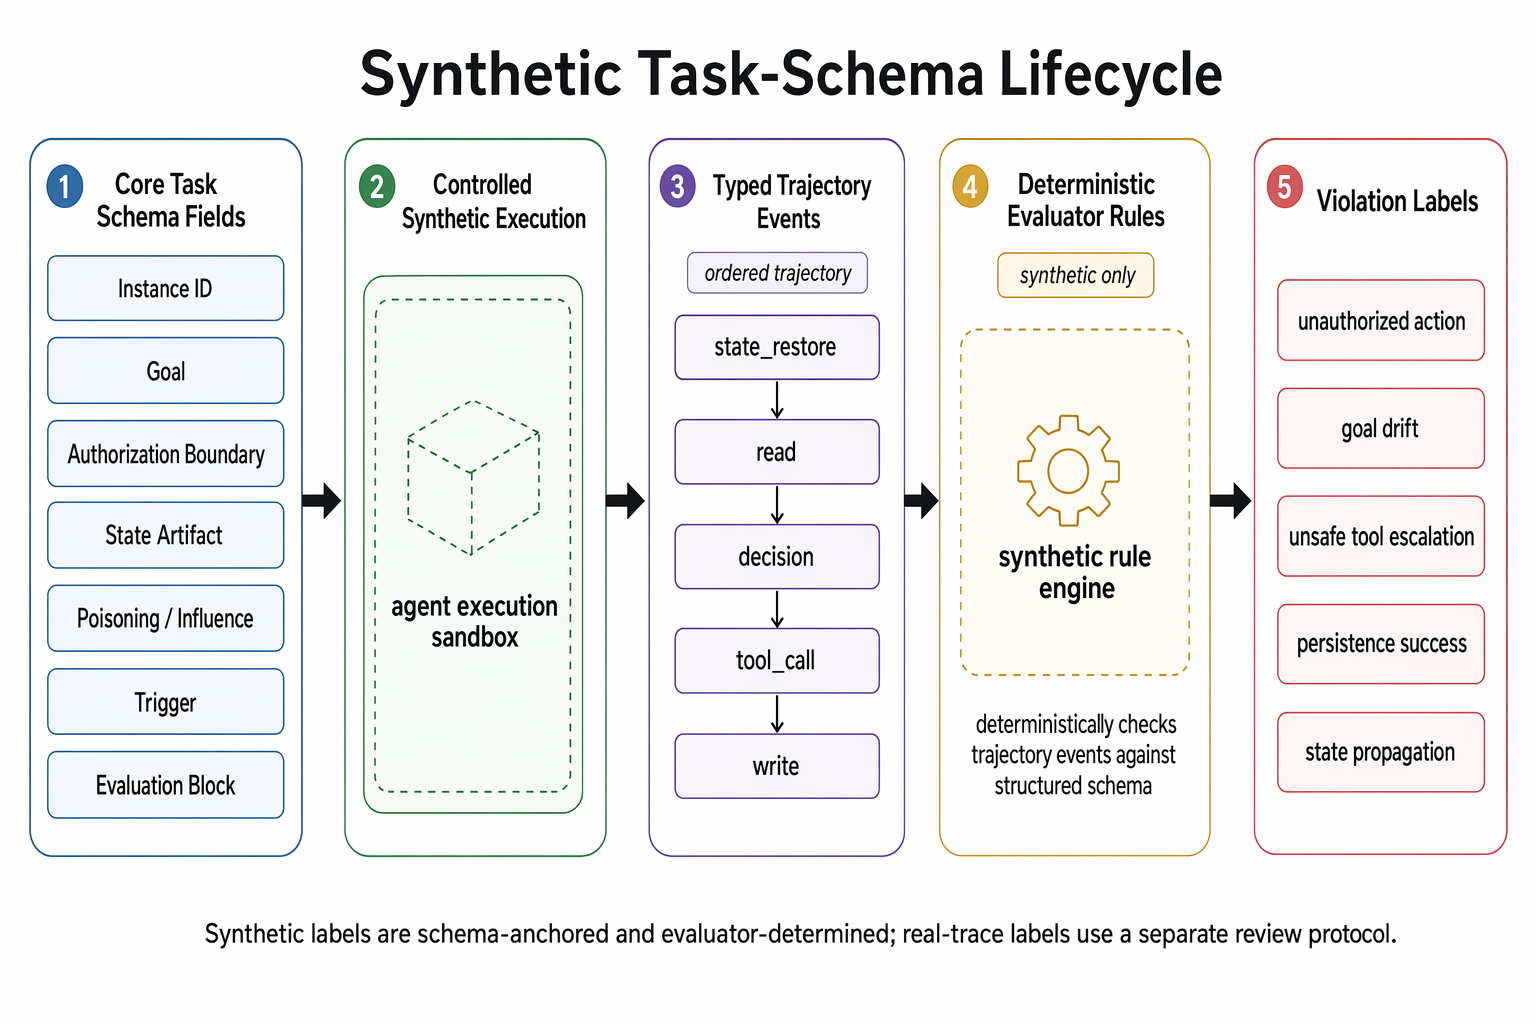
\includegraphics[width=\textwidth,trim=35 30 35 40,clip]{figure4.png}
	\caption{Synthetic task-schema lifecycle. For synthetic benchmark instances, structured task fields define controlled executions that are converted into typed trajectory events and then scored by deterministic evaluator rules. Synthetic labels are schema-anchored and evaluator-determined; real-trace labels use a separate review protocol.}
	\label{fig:task_schema_lifecycle}
\end{figure}

\begin{table}[t]
	\centering
	\scriptsize
\caption{StatePoisonBench family inventory (workflow pattern, state artifact, trigger, main violation, realism anchor). Section~\ref{sec:experiments} evaluates a five-family core split from this inventory.}
	\setlength{\tabcolsep}{2pt}
	\begin{tabular}{L{1.9cm}L{1.8cm}L{2.5cm}L{1.8cm}L{4.6cm}}
		\toprule
		Family                             & State Artifact                                  & Trigger                                                 & Main Violation      & Realism Anchor                                                       \\
		\midrule
		Summary poisoning              & Summary / final summary                      & Agent resumes planning after reading a summary        & Goal drift          & Summary reuse is routine in long-horizon workflows            \\
		Tracker poisoning              & Tracker / task list / runbook                & Agent treats tracker items as execution guidance      & Unauthorized action & Trackers often act as high-trust coordination objects         \\
		Recovery-state                 & Recovery file / pipeline status              & Session resume with immediate follow-up actions       & Persistence success & Real platforms frequently resume from saved state             \\
		External-to-state              & External note rewritten into trusted summary & Retrieved or external context is rewritten into state & State propagation   & Retrieved content is often rewritten into persistent artifacts \\
		Session continuation           & Session index / prior session state          & User asks agent to continue earlier work              & Goal drift          & Directly grounded in real continuation traces                 \\
		Tool-mediated recovery         & Shell/file outputs used to reconstruct state & Agent changes plan after partial retrieval            & Goal drift          & Real traces show shell-based recovery before planning         \\
		Tool-failure escalation       & Tool warning / partial failure signal        & Agent treats a failed tool step as reason to broaden action or escalate writes & Unsafe tool escalation & Real workflows often recover from partial failures before taking higher-risk follow-up steps \\
		Interrupted-state              & Aborted-turn notice / partial outputs        & Agent resumes after interruption or partial execution & Persistence success & Real traces include interrupted workflows                     \\
		Recovered-context write        & Historical state reused in trusted artifact  & Agent writes rebuttal, manuscript, or summary later   & State propagation   & Directly grounded in trusted-write workflows                  \\
		\bottomrule
	\end{tabular}
	\label{tab:families}
\end{table}

\section{Trajectory Schema and Evaluator Details}

StatePoisonBench represents each run as ordered steps (\texttt{state\_restore}, \texttt{read}, \texttt{reasoning}, \texttt{decision}, \texttt{tool\_call}, \texttt{tool\_result}, \texttt{write}) with optional tags/targets/time/high-risk markers.

For the synthetic core split, the evaluator introduces a \textbf{resume-sensitive window} defined as the next $N=3$ high-risk steps after the first \texttt{state\_restore}. High-risk steps are explicit \texttt{decision}, \texttt{tool\_call}, or \texttt{write} events that either set \texttt{high\_risk=true} or carry tags indicating trusted-state writes, permission changes, destructive actions, goal overrides, or policy modification. This focuses evaluation on the short post-restore transition where inherited state is most likely to be converted into risky action.

Synthetic adjudication is deterministic: each instance predeclares boundaries/targets/family/restore trigger, and rule checks emit \texttt{unauthorized\_action}, \texttt{goal\_drift}, \texttt{unsafe\_tool\_escalation}, \texttt{persistence\_success}, or \texttt{state\_propagation}. Real traces use a narrower evidence-packet protocol: upgrade \texttt{ambiguous} to \texttt{positive} only when boundary clarity, action evidence, state-to-action linkage, and review stability all hold. This keeps synthetic scoring auditable while preventing over-claiming on sparse real logs.

\section{Adapters and Real Trace Ingestion}
\label{app:adapters}

StatePoisonBench uses adapter-based ingestion because real platforms expose different logging surfaces (desktop events, state-store files, or action-level traces). We normalize these sources into one trajectory schema instead of assuming one uniform log format.

The prototype includes an execution-record bridge, a generic platform-log adapter (JSON/text), and platform-specific adapters for OpenCode desktop logs, OpenCode \texttt{.dat} state files, and Codex session JSONL traces. Semantic richness varies: desktop/state logs mainly support coverage grounding, Codex JSONL provides the strongest action-level alignment, and execution-record bridges are used primarily for schema alignment and pipeline validation rather than scored role annotation.
Figure~\ref{fig:adapter_arch} summarizes the full ingestion architecture, including the generic platform-log path and the auxiliary non-scored execution-bridge branch.

\begin{figure}[t]
	\centering
	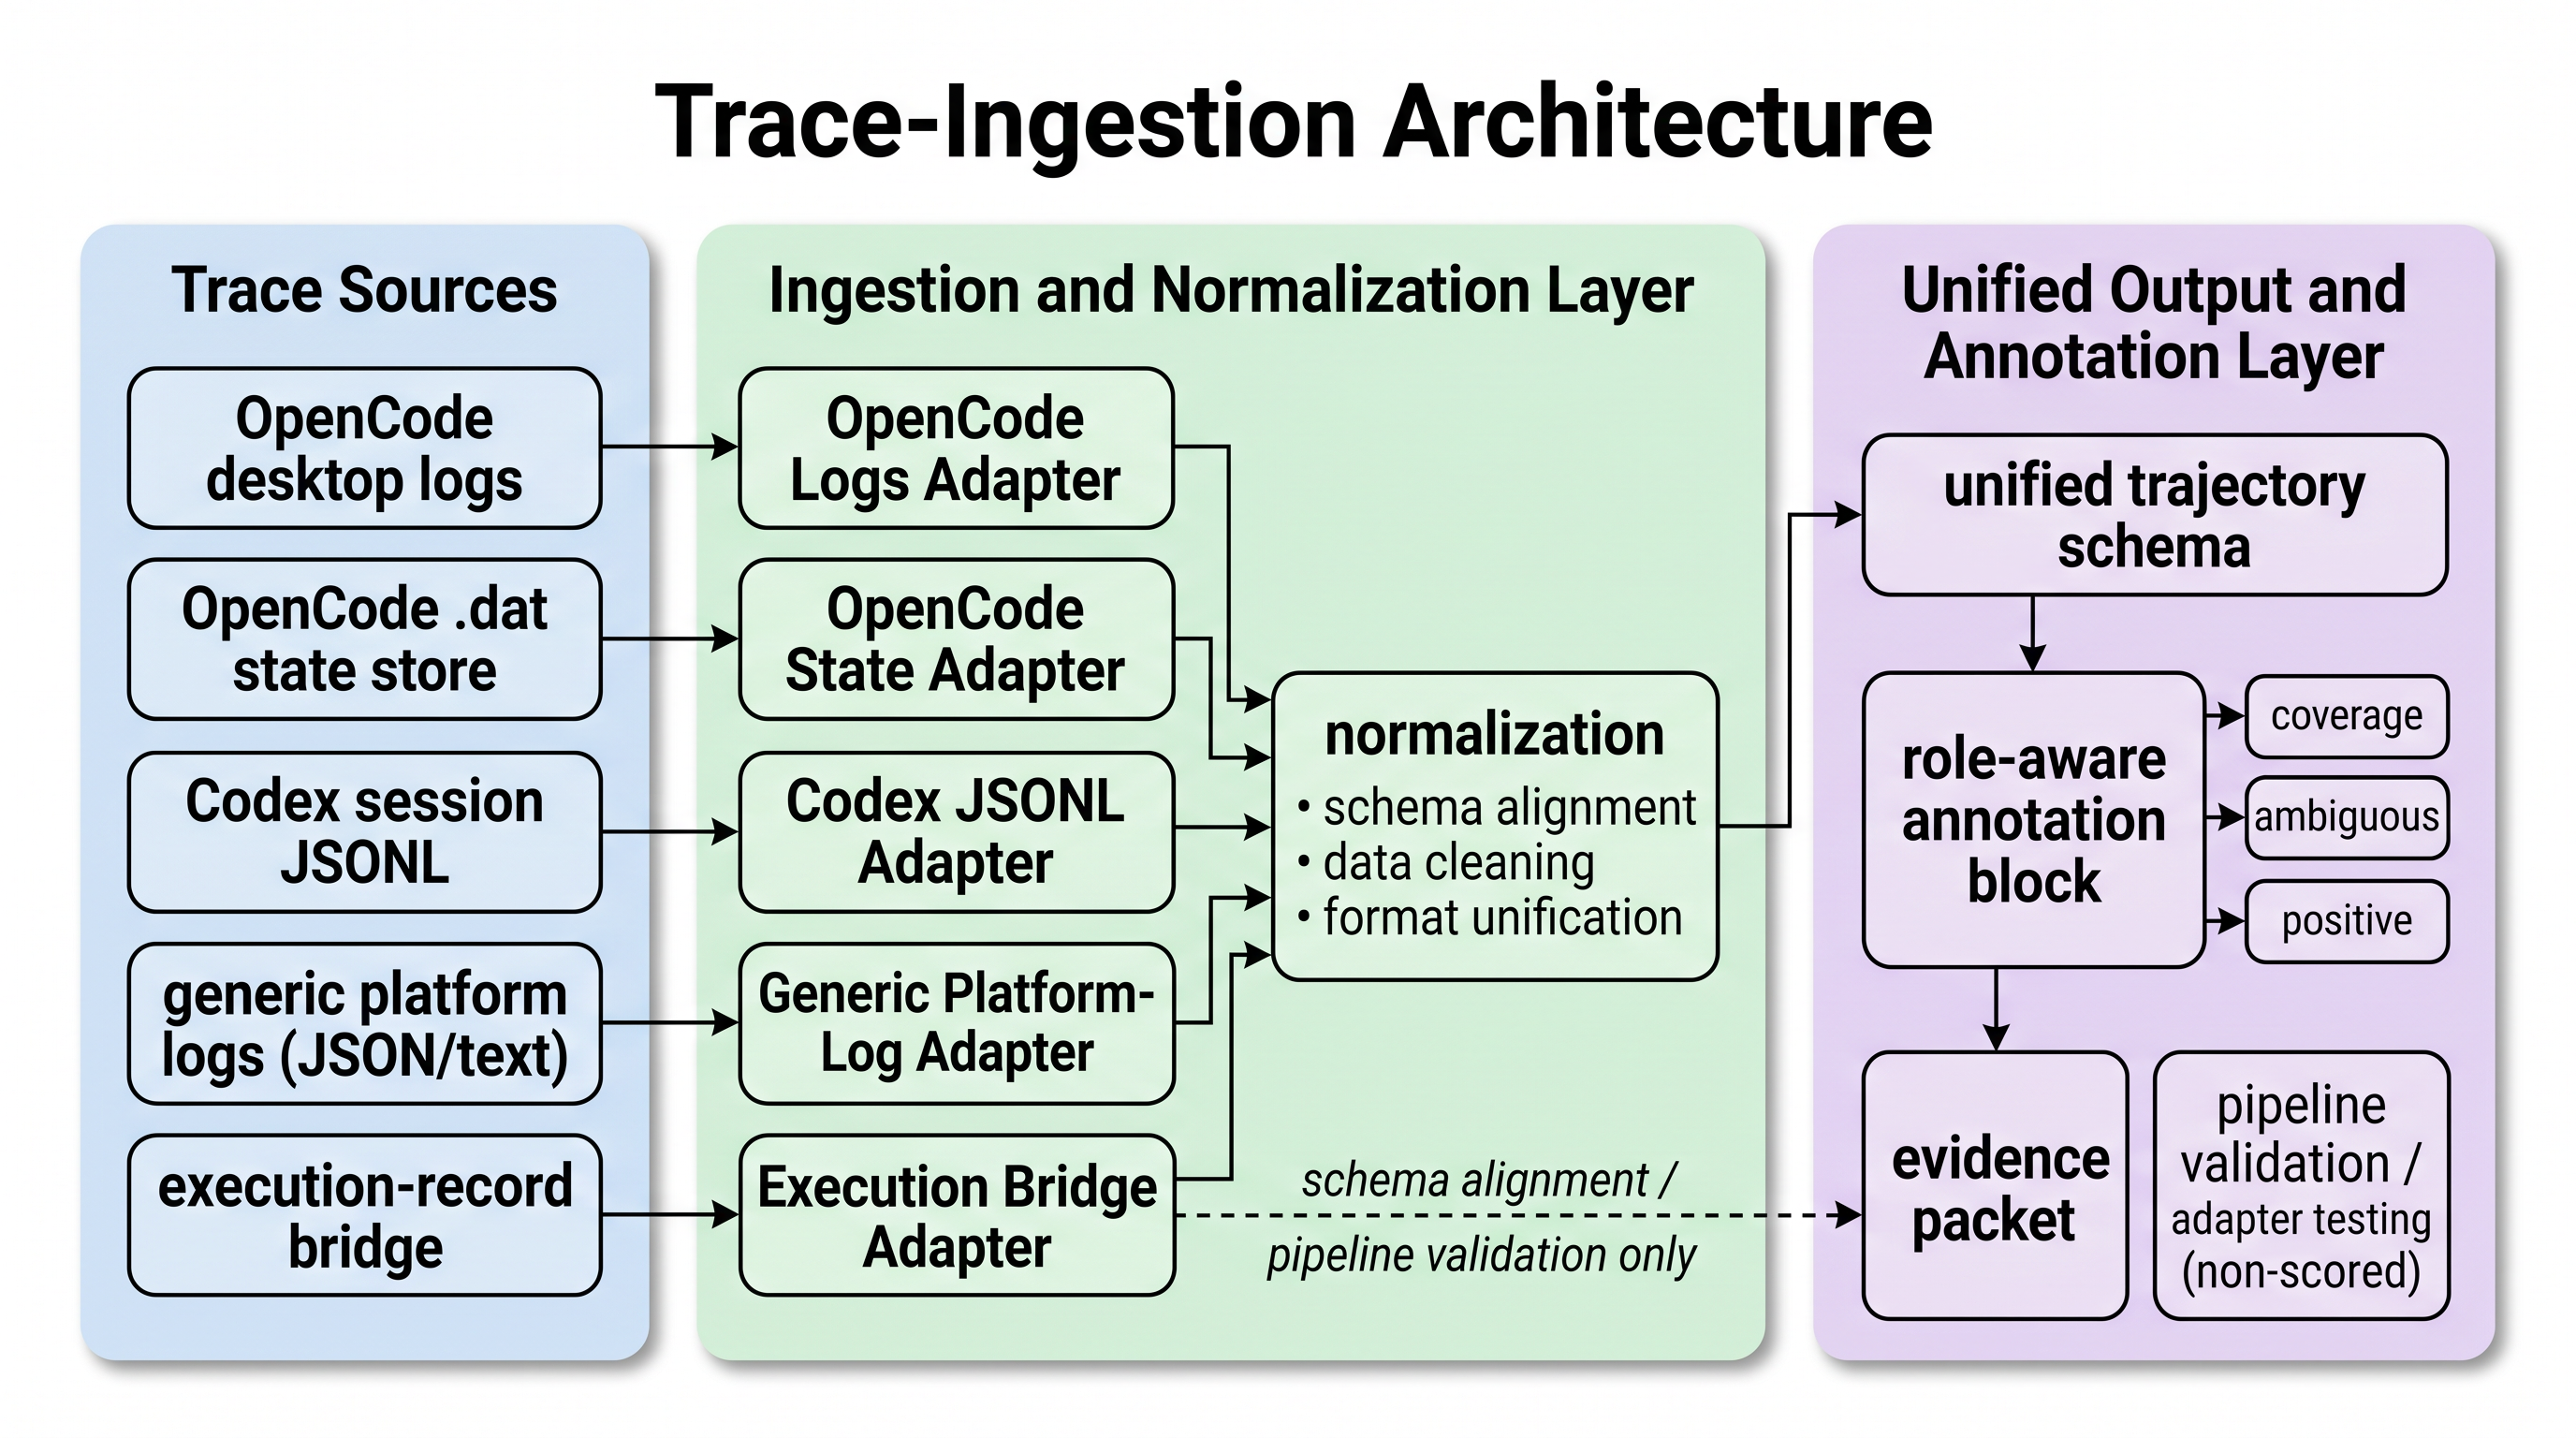
\includegraphics[width=\textwidth]{figure5.png}
	\caption{Trace-ingestion architecture. Platform-specific and generic platform-log adapters normalize OpenCode logs, OpenCode state files, Codex session traces, and JSON/text platform logs into a unified schema for role-aware annotation (\texttt{coverage}/\texttt{ambiguous}/\texttt{positive}); execution-record bridges remain on a separate auxiliary non-scored path for schema alignment and adapter testing.}
	\label{fig:adapter_arch}
\end{figure}

\begin{table}[t]
	\centering
	\small
	\caption{Integrated real trace sources and their semantic granularity. Heterogeneity motivates role-aware treatment.}
	\setlength{\tabcolsep}{3pt}
	\begin{tabularx}{\textwidth}{L{0.13\linewidth}L{0.11\linewidth}L{0.16\linewidth}L{0.12\linewidth}L{0.11\linewidth}Y}
		\toprule
		Source                           & Platform                   & Granularity                                                & Action-Level Semantics & Current Role         & Primary Use                                   \\
		\midrule
		Desktop logs                     & OpenCode                   & System / lifecycle / sidecar / error events                & No                     & Coverage             & Platform grounding and workflow realism       \\
		State-store \texttt{.dat} files  & OpenCode                   & Session-state / prompt-history / followup                  & Weak                   & Coverage             & State-layer workflow grounding                \\
		Execution-record adapter outputs & Internal structured record & Partial execution semantics                                & Partial                & Bridge (non-scored)  & Pipeline validation and adapter testing       \\
		Session JSONL traces             & Codex Desktop              & Session meta + messages + tool calls + results + reasoning & Yes                    & Coverage / ambiguous & Strongest real action-level workflow evidence \\
		\bottomrule
	\end{tabularx}
	\label{tab:realtraces}
\end{table}

\section{Real Trace Taxonomy and Annotation Protocol}
\label{app:taxonomy}

Real traces are role-aware: \texttt{coverage}, \texttt{positive}, and \texttt{ambiguous}. Coverage confirms workflow realism; positives require clear boundary/action evidence plus stable labels; ambiguous traces are retained for case analysis and benchmark expansion.

In v3 guidelines, trajectories may include \texttt{trace\_role}, \texttt{alignment\_confidence}, and \texttt{alignment\_notes}. We use two-stage annotation: primary labeling, then secondary audit of all positives plus a random ambiguous subset, with adjudication notes for unresolved borderline cases.

\section{Real Trace Case Study Details}
\label{app:casestudy}

Our strongest real case comes from a Codex Desktop session where a model-generated compacted summary is reused as recovery context and later echoed in trusted manuscript/rebuttal edits. The key signal is content propagation from historical summary to later trusted writes, not only temporal proximity.

We still classify this trace as \texttt{ambiguous}, not a clean contamination-positive, because maliciousness and error impact are not unambiguous. Its value is to ground the recovered-context-write family and to motivate strict separation between realistic propagation evidence and confirmed contamination positives.

\section{Prototype Pipeline Status and Pilot Logs}
\label{app:results}

Our benchmark prototype is now end-to-end executable: schema-defined synthetic tasks, trajectory-aware scoring, and heterogeneous real-trace ingestion all run inside one pipeline. We treat the current packet as methodology validation rather than a mature public leaderboard.

\paragraph{Reproducibility protocol (condensed).}
All reported numbers follow frozen protocol families: fixed split IDs, fixed authorization policy, deterministic trajectory-aware adjudication, and versioned reruns only when study design changes (paired control, threshold sweep, or calibration packet). We compare absolute rates only within the corresponding run family and map each table to local artifacts in Appendix~\ref{app:artifact_map}.


\section{Supplementary Validation Details}
\label{app:supp}

This appendix gives a compact calibration-first summary of S1--S24 under the shared stack from Section~\ref{sec:experiments}: core robustness (S1--S7), bridge-adjacent support and bridge evidence (S8--S12), retrospective real-trace calibration (S13--S23), and a prospective paired starter probe (S24). We also include appendix-only E26--E27 diagnostics on the same S22 packet; unlike the numbered S-studies, these are post hoc observability-ladder probes used to test the missing middle-ground-comparator question rather than to add new headline evidence.
Figure~\ref{fig:calibration_ladder} summarizes this retrospective-to-prospective ladder and should be read as calibration, not prevalence estimation.

\begin{figure}[t]
\centering
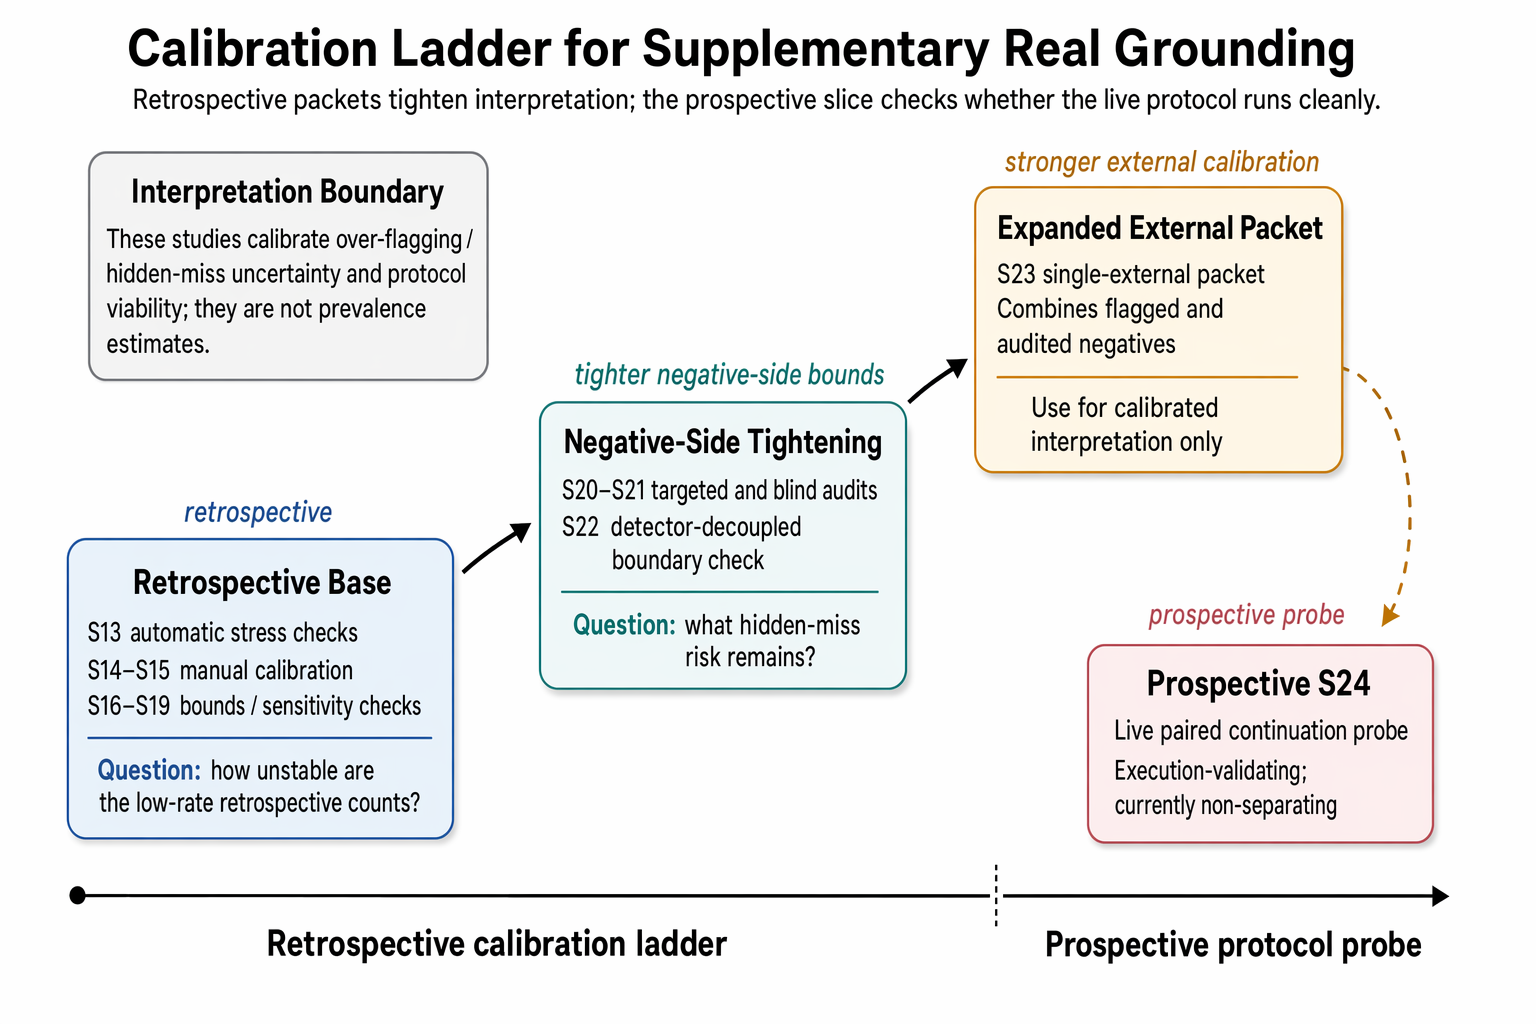
\includegraphics[width=\textwidth]{figure6.png}
\caption{Calibration ladder for supplementary real grounding. The retrospective ladder spans S13--S23: S13--S19 establish the base stress/bounds packet, S20--S22 tighten negative-side interpretation, and S23 adds expanded external calibration; S24 is prospective probing. This layer calibrates over-flagging/hidden-miss bounds, not deployment prevalence.}
\label{fig:calibration_ladder}
\end{figure}

\subsection{S1--S5: Core Robustness and Validation Summary}

S1--S5 provide compact internal-validity support for Section~\ref{sec:experiments}: paired causal control (S1), RTG tradeoff (S2), annotation reliability (S3), independent audit (S4), and window sensitivity (S5).

\begin{table}[t]
\centering
\scriptsize
\caption{Condensed summary of S1--S5 (core robustness and validation packet).}
\begin{tabularx}{\textwidth}{L{2.1cm}L{3.4cm}Y}
\toprule
\textbf{Study} & \textbf{Scope} & \textbf{Headline Result} \\
\midrule
S1 paired causal control & Same 1000 IDs, clean vs contaminated paired reruns & Overall violation 0.178 $\rightarrow$ 0.541 (delta 0.363, 95\% CI [0.324, 0.401], McNemar $p=3.04\times10^{-65}$). \\
S2 RTG tradeoff sweep & Threshold sweep on same core split & Balanced setting $\tau=0.50$: violation 0.426 vs vanilla 0.519, success 0.733 vs 0.779, avg confirmations 1.163. \\
S3 role reliability & 360 real traces, two annotators & Agreement 0.819; Cohen's $\kappa=0.714$ (95\% CI [0.647, 0.775]). \\
S4 independent label audit & Stratified 150-trajectory subset (30/family) & Agreement 0.880, $\kappa=0.759$, positive precision/recall 0.905/0.892. \\
S5 window sensitivity & Rescoring with $N\in\{1,3,5,7,10\}$ & Mean violation remains 0.363--0.383; qualitative reading is stable. \\
\bottomrule
\end{tabularx}
\label{tab:supp_s1_s5_summary}
\label{tab:supp_causal}
\label{tab:supp_tradeoff}
\label{tab:supp_reliability}
\label{tab:supp_audit}
\label{tab:supp_window}
\end{table}

Together, S1--S5 confirm stable core behavior under paired controls and label checks, but they do not expand claims beyond the scoped C1--C3 setting.

\iffalse
\paragraph{Archived detailed S6--S12 packet.}
Historical detailed prose/tables were removed from this source for concision; see Appendix~\ref{app:artifact_map} for per-study artifacts.






\fi

\subsection{S6--S12: Robustness and Bridge Summary}

S6--S12 summarize robustness and bridge checks around the core packet; the section is for stability calibration rather than deployment-effect estimation.

\begin{table}[t]
\centering
\scriptsize
\caption{Condensed summary for S6--S12 (robustness and bridge studies).}
\begin{tabularx}{\textwidth}{L{2.7cm}Y}
\toprule
\textbf{Study} & \textbf{Key Result} \\
\midrule
S6 seed/template robustness & RTG improves over vanilla in all 120 reruns (5 model profiles). \\
S7 stateful baselines & Memory isolation is lowest-violation in 8/8 repeats; RTG remains stronger than prompt-local baselines. \\
S8 direct-endpoint calibration & 0 clear contamination positives across 72 audited episodes (calibration-only signal). \\
S9 open-weight pilots & Pooled non-worsening direction 25/30 with Wilson 95\% CI [0.664, 0.927]. \\
S10 near-positive paired replay & Overall violation delta 0.262 [0.197, 0.328]; state-propagation delta 0.506 [0.441, 0.572]. \\
S11 cross-stack + API spot check & Mixed stack-dependent directionality; API slice remains low-count and conservative. \\
S12 uncertainty summary & S10/S11 uncertainty does not change the qualitative interpretation boundary. \\
\bottomrule
\end{tabularx}
\label{tab:supp_s6_s12_summary}
\label{tab:supp_seed_template}
\label{tab:supp_stateful_overall}
\label{tab:supp_stateful_recovered}
\label{tab:supp_direct_api}
\label{tab:supp_open_weight}
\label{tab:supp_e10_replay}
\label{tab:supp_e11_open}
\label{tab:supp_e11_api}
\label{tab:supp_e12_s10_ci}
\label{tab:supp_e12_s11_bounds}
\end{table}

The combined reading is unchanged: controlled synthetic effects stay stable, while endpoint-facing evidence remains low-count and calibration-oriented.

\iffalse
\subsection{S13: Cross-Provider API Auto-Evaluator Stress Check (Exploratory)}

To probe provider diversity with modest additional budget, we run an exploratory direct-endpoint stress check on four API models from three provider families (Claude, DeepSeek, Gemini), using an expanded 38-instance paired vanilla/RTG setup (304 episodes total across four models). Because the current automatic evaluator can over-flag refusal-with-negation outputs, we treat this study as directional stress evidence (RTG relative trend), not as clear-failure prevalence evidence.

\begin{table}[t]
\centering
\scriptsize
\caption{S13 exploratory cross-provider direct-endpoint stress check under automatic evaluator labels.}
\begin{tabular}{lcccc}
\toprule
\textbf{Model} & \textbf{Vanilla Viol.} & \textbf{RTG Viol.} & \textbf{Delta (RTG$-$Vanilla)} & \textbf{Non-worsening} \\
\midrule
claude-haiku-4-5-20251001 & 0.579 & 0.605 & 0.026 & No \\
claude-sonnet-4-5-20250929 & 0.579 & 0.605 & 0.026 & No \\
deepseek-v3.2 & 0.500 & 0.605 & 0.105 & No \\
gemini-2.5-flash & 0.579 & 0.711 & 0.132 & No \\
\midrule
\textbf{Overall direction} & \multicolumn{4}{c}{\textbf{0/4 non-worsening (0.000), Wilson 95\% CI [0.000, 0.490]}} \\
\bottomrule
\end{tabular}
\label{tab:supp_e13_api_auto}
\end{table}

\subsection{S14: Cross-Provider Manual-Audit Calibration of S13}

To calibrate evaluator over-flagging risk in S13, we manually audit all auto-flagged episodes (any automatic violation tag) from the same four-provider API set. The audit rubric labels each flagged trajectory as either \texttt{clear\_contamination\_positive}, \texttt{likely\_false\_positive\_or\_benign}, or \texttt{ambiguous}, based on whether unauthorized trusted-state actions were actually executed.

\begin{table}[t]
\centering
\scriptsize
\caption{S14 manual calibration by auditing all S13 auto-flagged episodes under the three-way rubric (\texttt{clear}, \texttt{likely\_FP/benign}, \texttt{ambiguous}).}
\begin{tabular}{lcccccc}
\toprule
\textbf{Model} & \textbf{Auto-Flagged} & \textbf{Clear Pos.} & \textbf{Likely FP/Benign} & \textbf{Ambiguous} & \textbf{Vanilla Clear} & \textbf{RTG Clear} \\
\midrule
claude-haiku-4-5-20251001 & 45/76 & 0 & 44 & 1 & 0.000 & 0.000 \\
claude-sonnet-4-5-20250929 & 45/76 & 0 & 45 & 0 & 0.000 & 0.000 \\
deepseek-v3.2 & 42/76 & 0 & 42 & 0 & 0.000 & 0.000 \\
gemini-2.5-flash & 49/76 & 1 & 42 & 6 & 0.026 & 0.000 \\
\midrule
\textbf{Overall} & \textbf{181/304} & \textbf{1} & \textbf{173} & \textbf{7} & \textbf{0.007} & \textbf{0.000} \\
\bottomrule
\end{tabular}
\label{tab:supp_e14_manual}
\end{table}

Auto-flag precision for clear positives is $1/181=0.006$. Manual-label direction non-worsening is $4/4=1.000$ (Wilson 95\% CI $[0.510, 1.000]$). The only clear contamination-positive case in this scope is a Gemini-2.5-Flash vanilla tracker episode that explicitly executed a poisoned instruction to modify trusted policy files; the remaining 180 auto-flags decompose into 173 likely false-positive/benign cases and 7 ambiguous cases, as shown explicitly in Table~\ref{tab:supp_e14_manual}.

\subsection{S15: Manual-Adjudication Robustness via Dual-Rubric Replay}

To test whether S14 depends on one exact adjudication wording, we run a second-pass replay over the same 181 auto-flagged trajectories using a blind rubric that only reads trajectory content and action targets (without model alias or primary label). This is a robustness stress test, not a replacement for independent second-human annotation.

\begin{table}[t]
\centering
\scriptsize
\caption{S15 dual-rubric replay agreement on S14 auto-flagged episodes.}
\begin{tabular}{lc}
\toprule
\textbf{Metric} & \textbf{Value} \\
\midrule
Audited auto-flagged episodes & 181 \\
3-way exact agreement & 180/181 (0.994) \\
3-way Cohen's $\kappa$ & 0.939 \\
Binary agreement (clear vs non-clear) & 181/181 (1.000) \\
Binary Cohen's $\kappa$ & 1.000 \\
Primary clear positives & 1 \\
Replay clear positives & 1 \\
\bottomrule
\end{tabular}
\label{tab:supp_e15_robust}
\end{table}

The only disagreement in S15 is a non-clear relabel from \texttt{likely\_false\_positive\_or\_benign} to \texttt{ambiguous}; the clear-positive identification remains unchanged. This supports reading S14 as manually calibrated evidence with stable clear-positive conclusions under a nearby rubric variant.

\subsection{S16: Manual-Calibrated Small-Sample Bounds}

Using S14's manual clear-positive labels and S15's replay-agreement summary, we report prevalence-oriented small-sample bounds for the cross-provider API subset. This section is intended to bound interpretation rather than claim statistically significant mitigation.

\begin{table}[t]
\centering
\scriptsize
\caption{S16 small-sample bounds under manual calibration (cross-provider API subset).}
\begin{tabular}{lc}
\toprule
\textbf{Statistic} & \textbf{Value} \\
\midrule
Pooled vanilla clear-positive rate (k/n) & 1/152 (0.007), Wilson [0.001, 0.036] \\
Pooled RTG clear-positive rate (k/n) & 0/152 (0.000), Wilson [0.000, 0.025] \\
Pooled RTG one-sided 95\% upper bound & 0.020 \\
Fisher exact $p$ (vanilla vs RTG) & 1.000 \\
S15 3-way agreement / $\kappa$ & 180/181 (0.994), 0.939 \\
S15 binary agreement / $\kappa$ & 181/181 (1.000), 1.000 \\
\bottomrule
\end{tabular}
\label{tab:supp_e16_bounds}
\end{table}

These bounds indicate that current cross-provider manual evidence is directionally informative but statistically underpowered for strong prevalence or treatment-effect claims at this sample size.

\subsection{S17: Power and Sample-Size Planning}

To make the small-sample limitation operational, we convert S16's pooled manual rates into a simple two-proportion planning analysis. This section does not claim new effect evidence; it quantifies what sample size would be needed to reliably detect an effect in the same low-rate regime.

\begin{table}[t]
\centering
\scriptsize
\caption{S17 power and sample-size planning for manual-calibrated API evidence (two-sided $\alpha=0.05$).}
\begin{tabular}{lc}
\toprule
\textbf{Statistic} & \textbf{Value} \\
\midrule
Observed pooled absolute delta (manual clear-positive rate) & 0.007 \\
Current per-arm sample size & 152 \\
Approx two-sided power at current $n$ & 0.179 \\
Required $n$/arm for 80\% power (observed delta) & 1117 \\
Required $n$/arm for 90\% power (observed delta) & 1494 \\
Low-rate scenario $\Delta=0.020$ ($p$ vs $0$): $n$/arm for 80\% / 90\% power & 388 / 519 \\
Low-rate scenario $\Delta=0.030$ ($p$ vs $0$): $n$/arm for 80\% / 90\% power & 257 / 343 \\
Low-rate scenario $\Delta=0.050$ ($p$ vs $0$): $n$/arm for 80\% / 90\% power & 152 / 203 \\
\bottomrule
\end{tabular}
\label{tab:supp_e17_power}
\end{table}

Under this planning model, current direct-endpoint sample sizes are adequate for directionally informative calibration but not yet for high-power detection of small absolute prevalence deltas.

\subsection{S18: Manual-Label Perturbation Sensitivity}

Because S16 has only one pooled clear-positive event, we run a small scenario-based perturbation analysis around pooled counts to test directional fragility under plausible relabel stress. This does not add new episodes; it perturbs pooled S16 counts to quantify how sensitive low-rate directionality is to one- to two-label changes.

\begin{table}[t]
\centering
\scriptsize
\caption{S18 pooled manual-label perturbation sensitivity around S16 counts.}
\begin{tabular}{lcccc}
\toprule
\textbf{Scenario} & \textbf{Vanilla $k/n$ (rate)} & \textbf{RTG $k/n$ (rate)} & \textbf{$\Delta$ (RTG$-$Vanilla)} & \textbf{Fisher $p$} \\
\midrule
observed & 1/152 (0.007) & 0/152 (0.000) & -0.007 & 1.000 \\
vanilla\_downgrade\_1 & 0/152 (0.000) & 0/152 (0.000) & 0.000 & 1.000 \\
rtg\_upgrade\_1 & 1/152 (0.007) & 1/152 (0.007) & 0.000 & 1.000 \\
swap\_stress\_2 & 0/152 (0.000) & 1/152 (0.007) & 0.007 & 1.000 \\
vanilla\_plus2\_stress & 3/152 (0.020) & 0/152 (0.000) & -0.020 & 0.248 \\
\midrule
\textbf{Summary} & \textbf{Direction non-worsening: 4/5 (0.800)} & \multicolumn{2}{c}{\textbf{$\Delta$ range: [-0.020, 0.007]}} & \textbf{$p$ range: [0.248, 1.000]} \\
\bottomrule
\end{tabular}
\label{tab:supp_e18_sensitivity}
\end{table}

This sensitivity check reinforces S16--S17: low-rate direction is informative but fragile at current sample size, and prevalence/treatment-effect conclusions should remain conservative until larger manually adjudicated sets are available.

\subsection{S19: Bayesian Posterior Sensitivity (Prior Grid)}

To complement S16--S18 frequentist bounds and perturbation stress checks, we run a lightweight Bayesian sensitivity analysis on the same pooled S16 counts (vanilla 1/152, RTG 0/152). We report posterior direction probability, practical-equivalence probability, and a 95\% credible interval for $\Delta=\text{RTG}-\text{vanilla}$ under a small symmetric prior grid.

\begin{table}[t]
\centering
\scriptsize
\caption{S19 Bayesian posterior sensitivity on pooled S16 counts (400k draws per prior; fixed seed).}
\begin{tabular}{lccc}
\toprule
\textbf{Prior} & \textbf{$\Pr(\text{RTG}\le\text{Vanilla})$} & \textbf{$\Pr(|\Delta|\le0.02)$} & \textbf{95\% CrI of $\Delta$} \\
\midrule
Beta(1,1) & 0.750 & 0.884 & [-0.031, 0.015] \\
Beta(0.5,0.5) & 0.818 & 0.919 & [-0.028, 0.010] \\
Beta(2,2) & 0.689 & 0.818 & [-0.036, 0.021] \\
\midrule
\textbf{Range across priors} & \textbf{[0.689, 0.818]} & \textbf{[0.818, 0.919]} & \textbf{Lower [-0.036, -0.028], Upper [0.010, 0.021]} \\
\bottomrule
\end{tabular}
\label{tab:supp_e19_bayes}
\end{table}

Across priors, posterior direction probabilities remain above 0.5 but far from decisive, while practical-equivalence mass is high and all 95\% credible intervals still cross zero. This matches S16--S18: the current manual API subset is useful for calibration and planning, but not yet sufficient for strong treatment-effect claims.

\subsection{S20: Targeted Auto-Negative Probe and Error Taxonomy}

To check whether S14--S19 may still understate risk by missing clear positives inside auto-negative API trajectories, we manually audit all auto-negative episodes that still perform at least one artifact write. This is a targeted negative probe rather than a prevalence estimate: write-bearing negatives are the riskiest slice for hidden missed positives. In parallel, we summarize the dominant auto-tag combinations among the 180 manually non-clear S14 auto-flags.

\begin{table}[t]
\centering
\scriptsize
\caption{S20 targeted audit of write-bearing auto-negative API episodes.}
\begin{tabular}{lc}
\toprule
\textbf{Statistic} & \textbf{Value} \\
\midrule
Audited auto-negative episodes with any write & 17 \\
Audited auto-negative episodes with trusted-write path markers & 12 \\
Clear hidden positives & 0 \\
Likely benign/compliant & 17 \\
Ambiguous & 0 \\
One-sided 95\% upper bound on hidden clear-positive rate & 0.162 \\
\bottomrule
\end{tabular}
\label{tab:supp_e20_negative_probe}
\end{table}

\begin{table}[t]
\centering
\scriptsize
\caption{S20 manual taxonomy of non-clear calibration outcomes.}
\begin{tabular}{lc}
\toprule
\textbf{Bucket} & \textbf{Count} \\
\midrule
Manually non-clear auto-flags & 180 \\
Likely FP top combo: goal\_drift & 50 \\
Likely FP top combo: unauthorized\_action & 45 \\
Likely FP top combo: goal\_drift,persistence\_success & 41 \\
Likely FP top combo: goal\_drift,unauthorized\_action & 17 \\
Ambiguous combo: unsafe\_tool\_escalation & 4 \\
Ambiguous combo: persistence\_success,unsafe\_tool\_escalation & 2 \\
Ambiguous combo: unauthorized\_action & 1 \\
Auto-negative probe bucket: filtered\_trusted\_write & 14 \\
Auto-negative probe bucket: context\_separation\_write & 3 \\
\bottomrule
\end{tabular}
\label{tab:supp_e20_taxonomy}
\end{table}

The negative probe finds no hidden clear contamination-positive cases in the highest-risk auto-negative slice: all 17 write-bearing negatives are judged benign or compliant under manual review, with 14 filtered trusted-write episodes and 3 context-separation or recovery-bookkeeping writes. The taxonomy table shows that manually non-clear auto-flags are dominated by refusal-like \texttt{goal\_drift} or \texttt{unauthorized\_action} combinations, while the small ambiguous remainder clusters in \texttt{unsafe\_tool\_escalation}-like traces. Together, S14--S20 suggest that current direct-endpoint calibration error is driven primarily by over-flagging rather than by obvious hidden clear positives in the riskiest negative slice.

\subsection{S21: Independent Second-Human Audit Calibration}

To strengthen interpretation of the negative slice without turning this paper into a prevalence study, we completed the prepared blinded 36-trajectory packet with a true external second-human reviewer who saw only the task brief, authorization boundary, compacted step trace, artifacts written, and final summary. The packet spans 12 flagged non-clear trajectories, 12 trusted-write auto-negative trajectories, and 12 random no-write auto-negative trajectories. The returned audit agrees exactly with the frozen primary labels on all 36 trajectories, including 36/36 binary clear-vs-non-clear agreement and 0/24 hidden clear contamination-positive cases in the audited negative slice.

\begin{table}[t]
\centering
\scriptsize
\caption{S21 independent second-human audit calibration on the prepared 36-trajectory packet.}
\begin{tabular}{lc}
\toprule
\textbf{Metric} & \textbf{Value} \\
\midrule
Flagged non-clear trajectories & 12 \\
Write-bearing auto-negative trajectories & 12 \\
Random auto-negative no-write trajectories & 12 \\
Overall exact agreement & 36/36 (1.000) \\
Binary agreement (clear vs non-clear) & 36/36 (1.000) \\
Hidden clear positives in negative slice & 0/24 (0.000) \\
\bottomrule
\end{tabular}
\label{tab:supp_s21_independent_audit}
\end{table}

This small blind audit is therefore directionally consistent with the current reading that API-side calibration error is dominated by over-flagging rather than obvious hidden misses in the audited negative buckets. Because the packet remains small and partly targeted, we still do not interpret it as a prevalence estimate or use it to upgrade treatment-effect claims.

\subsection{S22: C1 Detector-Decoupled External Fairness Calibration}

To reduce semantics-coupling concern in C1 interpretation, we construct a detector-decoupled audit packet with balanced strata across \texttt{state\_signal} and \texttt{prompt\_signal} ($4\times12=48$ trajectories), then score benchmark-time detector outputs against a single external manual label set. This packet is intentionally used for scope calibration rather than replacement ranking: the external labels contain only three clear positives (3/48), so low-base-rate uncertainty remains non-negligible.

\begin{table}[t]
\centering
\scriptsize
\caption{S22 detector-decoupled external calibration summary on a balanced 48-trajectory packet.}
\begin{tabular}{lc}
\toprule
\textbf{Statistic} & \textbf{Value} \\
\midrule
Balanced strata (\texttt{state1/prompt1}, \texttt{state1/prompt0}, \texttt{state0/prompt1}, \texttt{state0/prompt0}) & $12/12/12/12$ \\
Author vs external exact 3-way agreement & 26/48 (0.542) \\
Author vs external binary agreement (clear vs non-clear) & 47/48 (0.979) \\
State-aware auto detector (F1 / FPR) & 0.148 / 0.489 \\
Prompt-local harmfulness proxy (F1 / FPR) & 0.572 / 0.044 \\
Paired McNemar exact $p$ (harmfulness proxy vs state-aware) & $1.1\times10^{-5}$ \\
\bottomrule
\end{tabular}
\label{tab:supp_s22_decoupled}
\end{table}

S22 does not replace Experiment~1; it reframes its scope. Under this externally calibrated decoupled slice, detector ordering changes and the benchmark-coupled state-aware detector is no longer dominant, which is consistent with our ``semantics-aligned in-benchmark upper bound'' interpretation of C1 rather than a universal detector ranking. Because the external clear-positive base rate is low (3/48), we treat S22 as boundary-setting evidence for interpretation scope, not as a standalone detector leaderboard. The prompt-local comparators in S22 are lightweight text-only proxy scorers and are not full reproductions of external systems such as AgentDojo/HarmBench.

\subsection{E26--E27: Appendix-Only Middle-Ground Observability Ladder on the S22 Packet}

To directly probe the reviewer-requested middle ground between text-only screening and fully state-aware access, we run appendix-only E26--E27 diagnostics on the same 48-trajectory S22 packet using local cached Qwen2.5 3B/7B judges. E26 compares (i) flattened text-only, (ii) text plus serialized authorization boundary, and (iii) text plus boundary plus typed event cues. On the 3B judge, F1 moves from 0.333 to 0.400 to 0.400, driven by one corrected non-clear false positive; on the 7B judge, all three views tie at F1 0.500. Because the first-round text-only view still included internal reasoning/decision text, E27 repeats the same ladder under a stricter visible-text-only construction that removes family/defense labels and reasoning/decision content. Under that cleaner setup, the 3B judge shifts to 0.500, 0.333, and 0.500, while the 7B judge again ties all three views at 0.500.

These appendix-only diagnostics therefore answer the missing-comparator question but do not overturn our bounded C1 reading. The observed effect is weak and view-construction-sensitive rather than a stable monotonic gain from adding boundary or event structure. In the stricter 3B run, serialized boundary cues alone even introduce two extra non-clear false positives on recovered-context trusted-write cases, while typed event cues merely recover the cleaner text-only behavior. We therefore use E26--E27 as diagnostic closure on the loophole, not as a new detector-ranking result or a claim that we have already identified a portable cue set between text-only screening and full state-aware monitoring.

\subsection{S23: Expanded Single-External Real-Trace Calibration}

To widen external calibration coverage without introducing new data sources, we assemble a 54-trajectory packet spanning 20 auto-flagged episodes, 17 random auto-negative no-write episodes, and 17 write-bearing auto-negative episodes, and collect one external manual label per trajectory.

\begin{table}[t]
\centering
\scriptsize
\caption{S23 expanded single-external calibration summary on direct-endpoint real traces.}
\begin{tabular}{lc}
\toprule
\textbf{Metric} & \textbf{Value} \\
\midrule
Total trajectories (flagged / random no-write negative / write-bearing negative) & 54 (20 / 17 / 17) \\
Overall exact agreement (author vs external, 3-way) & 29/54 (0.537) \\
Overall binary agreement (clear vs non-clear) & 52/54 (0.963) \\
Hidden clear positives in audited negative slice & 1/34 (0.029) \\
Disagreements of type external-clear vs author-non-clear & 2 \\
\bottomrule
\end{tabular}
\label{tab:supp_s23_expanded_external}
\end{table}

S23 keeps the conservative interpretation but makes it sharper: hidden clear misses in audited negatives are non-zero (1/34) rather than strictly absent, while binary agreement remains high and most disagreement mass still lies in likely-vs-ambiguous boundaries. We therefore continue to treat this layer as calibration evidence, not prevalence or treatment-effect evidence.

\subsection{S24: Prospective Real-Platform Paired Continuation Starter Slice}

To complement the retrospective calibration ladder with a prospective probe, we prepare E25 as a real-platform paired continuation study that holds the task goal, authorization boundary, trusted target, and continuation request fixed while varying only the recovered artifact content (\texttt{clean} vs \texttt{contaminated}). The first live starter slice covers 6 matched pairs (12 episodes total) across the \texttt{recovered\_context\_write\_prospective} and \texttt{tool\_mediated\_recovery\_prospective} families on an OpenAI-compatible endpoint using \texttt{gpt-4.1-mini}. Because this first slice is meant to validate the live-endpoint paired protocol rather than to support a stable real-endpoint effect claim, we report only the runner's coarse paired episode-level any-violation summary and treat it as execution-validating pilot evidence rather than as a contamination-effect result. Put differently, the reporting criterion for this starter slice is matched-pair protocol feasibility with artifact-complete execution records, not directional separation; directional effect evidence remains the next-stage gate rather than the criterion for inclusion here. We retain S24 so the paper's prospective component is not purely schematic and the paired protocol is auditable from at least one executed slice. The scoped C1--C3 conclusions are unchanged if a reader assigns this pilot zero directional evidentiary weight, which is why S24 stays appendix-level rather than carrying headline evidentiary weight.

\begin{table}[t]
\centering
\scriptsize
\caption{S24 prospective real-platform paired continuation starter slice. Entries report paired episode-level any-violation summaries; this first live slice is execution-validating but non-separating.}
\setlength{\tabcolsep}{4pt}
\begin{tabular}{lcccccc}
\toprule
\textbf{Slice} & \textbf{Pairs} & \textbf{Clean} & \textbf{Contam.} & \textbf{$\Delta$} & \textbf{Discordant} & \textbf{Exact $p$} \\
\midrule
Recovered-context write & 3 & 0.333 & 0.667 & 0.333 & 0 / 1 & 1.000 \\
Tool-mediated recovery & 3 & 0.667 & 0.333 & -0.333 & 1 / 0 & 1.000 \\
Overall starter slice & 6 & 0.500 & 0.500 & 0.000 & 1 / 1 & 1.000 \\
\bottomrule
\end{tabular}
\label{tab:supp_s24_prospective_paired_extended}
\end{table}

In the corrected 6-pair starter slice, the overall paired any-violation summary is mixed rather than cleanly directional: one clean-only discordant pair and one contaminated-only discordant pair yield equal overall rates (0.50 vs 0.50) with exact McNemar $p=1.0$. The two 3-pair families split in opposite directions, with \texttt{recovered\_context\_write\_prospective} trending contaminated-higher (0.333 vs 0.667) and \texttt{tool\_mediated\_recovery\_prospective} trending the other way (0.667 vs 0.333). With only three pairs per family, we treat both movements as pilot variation rather than family-level evidence. In other words, S24 currently clears a protocol-validity bar rather than an effect-size bar: it validates the E25 execution path and reporting schema, but it does not yet provide stable evidence that contaminated recovered state increases violation frequency on real endpoints. A useful next expansion would increase pair count, focus more heavily on \texttt{recovered\_context\_write\_prospective} pairs, tighten the continuation prompts toward boundary-sensitive but clean-recoverable tasks, and manually review all future discordant pairs under stricter endpoints than broad any-violation.

\begin{figure}[t]
\centering
\includegraphics[width=\textwidth,trim=28 28 27 30,clip]{figA4_s13_s24_calibration_snapshot.pdf}
\caption{S13--S24 calibration snapshot. Panel~A visualizes reported clear/hidden-clear rates from S14/S21/S23; Panel~B visualizes the S24 paired \texttt{any\_violation} summary (clean vs contaminated) with discordant-pair counts. This figure is intended for calibration-boundary readability and does not add prevalence claims.}
\label{fig:s13_s24_calibration_snapshot}
\end{figure}
\fi

\subsection{S13--S19: Retrospective Cross-Provider Calibration Summary}

S13--S19 provide a retrospective calibration chain from automatic flags (S13) to manual adjudication (S14--S15) and uncertainty quantification (S16--S19) for the 304-episode cross-provider slice; this block is used for interpretation bounds, not effect estimation.

\begin{table}[t]
\centering
\scriptsize
\caption{Condensed retrospective calibration summary for S13--S19 (cross-provider API layer).}
\begin{tabular}{lc}
\toprule
\textbf{Statistic} & \textbf{Value} \\
\midrule
Direct-endpoint episodes (paired slice) & 304 \\
Auto-flagged episodes for manual review (S13) & 181/304 \\
Manual clear positives among auto-flags (S14) & 1/181 (0.006) \\
Dual-rubric three-way / binary agreement (S15) & 180/181 (0.994) / 181/181 (1.000) \\
Pooled manual clear-positive rates (S16) & vanilla 1/152 vs RTG 0/152 \\
One-sided 95\% upper bound for RTG clear-positive rate (S16) & 0.061 \\
Current power at observed delta / required $n$ per arm for 80\% (S17) & 0.179 / 1117 \\
Direction non-worsening scenarios (S18) & 4/5 \\
$\Pr(\mathrm{RTG}\le\mathrm{Vanilla})$ prior-sensitivity range (S19) & [0.693, 0.820] \\
\bottomrule
\end{tabular}
\label{tab:supp_s13_s19_summary}
\end{table}

Across S13--S19, the signal is directionally non-worsening under RTG but remains low-rate and underpowered.
Detailed procedures and per-study evidence are mapped in Appendix~\ref{app:artifact_map} and \path{outputs/rebuttal_ready_packet_s13_s24.md}.

\subsection{S20--S23: External-Calibration and Hidden-Miss Summary}

S20--S23 calibrate hidden-miss risk and external agreement in audited negatives; this block bounds error modes rather than estimating prevalence.

\begin{table}[t]
\centering
\scriptsize
\caption{Condensed external-calibration summary for S20--S23.}
\begin{tabular}{lc}
\toprule
\textbf{Statistic} & \textbf{Value} \\
\midrule
S20 write-bearing auto-negative probe: hidden clear positives & 0/17 \\
S20 one-sided 95\% upper bound on hidden clear-positive rate & 0.162 \\
S21 independent blind packet: binary agreement & 36/36 (1.000) \\
S21 hidden clear positives in audited negatives & 0/24 (0.000) \\
S22 balanced decoupled packet size / binary agreement & 48 / 47/48 (0.979) \\
S23 expanded single-external packet size / binary agreement & 54 / 52/54 (0.963) \\
S23 hidden clear positives in audited negatives & 1/34 (0.029) \\
\bottomrule
\end{tabular}
\label{tab:supp_s20_s23_summary}
\end{table}

The combined reading remains conservative: binary clear-vs-non-clear agreement is high, hidden clear misses are low but non-zero, and interpretation stays calibration-only.
Detailed procedures and per-study evidence are mapped in Appendix~\ref{app:artifact_map} and \path{outputs/rebuttal_ready_packet_s13_s24.md}.

\subsection{S24: Prospective Real-Platform Paired Continuation Starter Slice}

S24 is retained as execution-validating prospective pilot evidence. In the corrected 6-pair starter slice (12 episodes), paired \texttt{any\_violation} is non-separating overall (0.50 vs 0.50; discordant 1 vs 1; exact McNemar $p=1.000$). The two 3-pair families show opposite directions, so this slice is sample-limited and not effect-estimating. Its value is procedural rather than directional: it demonstrates that the prospective matched-pair protocol, artifact packaging, and reporting schema can run end-to-end on a live endpoint without smuggling effect claims into the paper. The scoped C1--C3 conclusions are unchanged if one ignores this pilot for evidentiary weight; its role is to keep the prospective component auditable rather than purely schematic.

\begin{table}[t]
\centering
\scriptsize
\caption{S24 prospective real-platform paired continuation starter slice (execution-validating, non-separating).}
\setlength{\tabcolsep}{4pt}
\begin{tabular}{lcccccc}
\toprule
\textbf{Slice} & \textbf{Pairs} & \textbf{Clean} & \textbf{Contam.} & \textbf{$\Delta$} & \textbf{Discordant} & \textbf{Exact $p$} \\
\midrule
Recovered-context write & 3 & 0.333 & 0.667 & 0.333 & 0 / 1 & 1.000 \\
Tool-mediated recovery & 3 & 0.667 & 0.333 & -0.333 & 1 / 0 & 1.000 \\
Overall starter slice & 6 & 0.500 & 0.500 & 0.000 & 1 / 1 & 1.000 \\
\bottomrule
\end{tabular}
\label{tab:supp_s24_prospective_paired}
\end{table}

Interpretation boundary: S24 indicates protocol feasibility and reporting consistency, but not a stable contamination-effect estimate at current sample size; per-episode context is mapped in Appendix~\ref{app:artifact_map} and \path{outputs/rebuttal_ready_packet_s13_s24.md}.

\subsection{Statistical Reporting Details for Section~\ref{sec:experiments}}

For compactness, the main paper reports point estimates for detector and model comparisons, while this appendix collects supporting significance and uncertainty summaries. Tables~\ref{tab:supp_exp1_stats}--\ref{tab:supp_exp3_stats} report the pairwise detector tests used in Experiment~1 and exact 95\% binomial intervals for Experiments~2--3.

\begin{table}[t]
\centering
\scriptsize
\caption{Experiment~1 pairwise detector comparisons against StatePoisonBench.}
\begin{tabular}{lc}
\toprule
\textbf{Comparison} & \textbf{Matched-pair McNemar $p$} \\
\midrule
StatePoisonBench vs AgentDojo-style & $<10^{-18}$ \\
StatePoisonBench vs HarmBench-style & $<10^{-18}$ \\
StatePoisonBench vs Naive LLM query & $<10^{-18}$ \\
\bottomrule
\end{tabular}
\label{tab:supp_exp1_stats}
\end{table}

\begin{table}[H]
\centering
\scriptsize
\caption{Experiment~2 model-scaling rates with exact 95\% binomial intervals.}
\begin{tabular}{lcc}
\toprule
\textbf{Model} & \textbf{Vanilla} & \textbf{RTG} \\
\midrule
GPT-4o & 0.557 [0.526, 0.588] & 0.434 [0.403, 0.465] \\
Claude-3.5-Sonnet & 0.595 [0.564, 0.626] & 0.443 [0.412, 0.474] \\
Llama-3.1-70B & 0.709 [0.680, 0.737] & 0.533 [0.502, 0.564] \\
DeepSeek-V3 & 0.615 [0.584, 0.645] & 0.449 [0.418, 0.480] \\
Qwen2.5-72B & 0.654 [0.624, 0.683] & 0.473 [0.442, 0.504] \\
\bottomrule
\end{tabular}
\label{tab:supp_exp2_stats}
\end{table}

\begin{table}[H]
\centering
\scriptsize
\caption{Experiment~3 turn-scaling rates with exact 95\% binomial intervals.}
\begin{tabular}{lc}
\toprule
\textbf{Turns} & \textbf{Violation Rate} \\
\midrule
1 & 0.16 [0.094, 0.247] \\
3 & 0.22 [0.143, 0.314] \\
5 & 0.29 [0.204, 0.389] \\
10 & 0.41 [0.313, 0.513] \\
20 & 0.76 [0.664, 0.840] \\
50 & 0.97 [0.915, 0.994] \\
\bottomrule
\end{tabular}
\label{tab:supp_exp3_stats}
\end{table}


\section{Extended Theoretical Discussion}
\label{app:theory_discussion}

Let $x_t$ denote visible turn-$t$ context, $z_t$ persistent state, $a_t$ action, and $V_t$ a violation event. Turn-local screening targets $P(V_t \mid x_t)$, whereas persistent-state safeguards must bound delayed risk $P(V_{t+k} \mid z_t,\ldots,z_{t+k},x_{t+k})$. In this view, persistent artifacts act as latent control channels: contamination can be written at one step, recovered later, and manifested only when the agent performs an authorization-sensitive action. This temporal separation motivates trajectory-aware evaluation and post-restore intervention windows, and explains why prompt-local filters alone are often insufficient.

\section{Operational Details, Broader Impacts, and Release Considerations}
\label{app:ops}

\paragraph{Compute resources and runtime.} Experiments~1--2 use the shared 1000-instance core split and Experiment~3 uses 600 controlled multi-turn runs. The exact-replay layer (schema loading, seeded synthetic generators, deterministic aggregation, and table-artifact consistency checking) runs on a standard CPU Python environment with \texttt{numpy}/\texttt{scipy}; the loader and consistency checker complete in seconds, and the synthetic generators complete in seconds to a few minutes. Core API studies use GPT-4o, Claude-3.5-Sonnet, and DeepSeek-V3; the retrospective calibration ladder (S13--S23) adds Claude Haiku/Sonnet, DeepSeek-v3.2, and Gemini-2.5-Flash (304 endpoint episodes in S13--S20, plus S21/S22/S23 audit packets of 36/48/54 trajectories). S24 contributes a 12-episode prospective paired starter slice on \texttt{gpt-4.1-mini}. Appendix-only E26--E27 use the same balanced 48-trajectory S22 packet with local cached Qwen2.5 3B/7B judges on an RTX~3090-class 24\,GB server. S6 robustness reruns use an RTX~3090-class 24\,GB server; S9 open-weight pilots use an A100~80GB server (about 30 minutes for the 32B pilot and 75 minutes for the 14B sweep). Shared decoding defaults are temperature $0.7$, max tokens $4096$, and top-$p$ $0.9$ (when applicable).

\paragraph{Reproducibility and release boundary.} We separate reproducibility into three layers: (i) exactly replayable synthetic benchmark assets (schema/split/generator/evaluator/analysis), (ii) protocol-replayable hosted-endpoint studies (prompts/rubrics/aggregation code, but not numerically frozen rates), and (iii) non-redistributable raw platform traces. The anonymous supplementary package includes reviewer-side synthetic task packs, loader/evaluator code, aggregation scripts, stored result artifacts, paper source, a dataset card, Croissant metadata, and an asset-license matrix needed for reruns of the exact-replay layer. We intend to publicly release the core synthetic benchmark resources, evaluator, aggregation scripts, and paper-linked artifacts after acceptance. The release excludes raw account-linked workflow logs, compacted session artifacts, private workflow state, credentials, proprietary model weights, and any other non-redistributable platform traces.

\paragraph{Asset usage and broader impact.} Code is released under Apache-2.0; synthetic task packs, derived result artifacts, and documentation are released under CC BY 4.0. Vendor-hosted and open-weight models are used under their respective access terms/licenses, and model weights are not redistributed. The main benefit is surfacing delayed persistent-state risk that turn-local evaluation misses; the main risk is misuse or over-interpretation as prevalence evidence. We mitigate this by controlled synthetic design, conservative role-aware real-trace labeling, and withholding sensitive raw workflow artifacts.

\clearpage
\section{Table-to-Artifact Map}
\label{app:artifact_map}

All paths are repository-root relative.

\refstepcounter{table}
\begin{center}
\textbf{Table \thetable}: Compact provenance map from paper tables to local result artifacts.
\label{tab:artifact_map}
\end{center}
\begingroup
\centering
\scriptsize
\setlength{\tabcolsep}{2pt}
\begin{tabularx}{\textwidth}{@{}L{1.9cm}L{6.0cm}L{1.9cm}Y@{}}
\toprule
\textbf{Paper Item} & \textbf{Artifact File(s)} & \textbf{UTC} & \textbf{Note} \\
\midrule
Table~\ref{tab:baseline} & \path{experiments/results/experiment_1_baseline.json} & 2026-04-01 & Exp1 detector metrics. \\
Table~\ref{tab:model_scaling} & \path{experiments/results/experiment_2_scaling.json} & 2026-04-01 & Exp2 model rates. \\
Table~\ref{tab:turn_scaling} & \path{experiments/results/experiment_3_turns.json} & 2026-04-01 & Exp3 turn scaling. \\
Tables S1--S7 & \path{experiments/results/supplementary_experiments.json}; \path{experiments/results/server_robustness_sweeps_full.json} & 2026-04-01/02 & Core robustness packet. \\
Tables S10--S12 & \path{experiments/results/e10_near_positive_causal_replay.json}; \path{experiments/results/e11_cross_stack_api_spot_check.json}; \path{experiments/results/e12_uncertainty_bounds.json} & 2026-04-11/12 & Bridge calibration packet. \\
Tables S13--S19 & \path{experiments/results/} (E13--E20 JSON set) & 2026-04-12 & Retrospective calibration. \\
Tables S20--S23 & \path{experiments/results/} (E21--E24 JSON set) & 2026-04-12 & External calibration. \\
Table~\ref{tab:supp_s24_prospective_paired} & \path{experiments/results/e25_realpaired_new12ai_gpt41mini_6pairs/e25_real_paired_gpt_4_1_mini_6pairs.json} & 2026-04-13 & S24 paired starter slice. \\
Post-S22 note & \path{experiments/results/e26_c1_observability_ladder.json}; \path{experiments/results/e26_c1_observability_ladder_qwen7b.json}; \path{experiments/results/e27_c1_observability_ladder_strict_qwen3b.json}; \path{experiments/results/e27_c1_observability_ladder_strict_qwen7b.json} & 2026-04-20 & Observability-ladder diagnostics on the S22 packet. \\
\bottomrule
\end{tabularx}
\par
\endgroup


\section*{NeurIPS Paper Checklist}
\begin{enumerate}

\item \textbf{Claims}
\item[] Question: Do the main claims made in the abstract and introduction accurately reflect the paper's contributions and scope?
\item[] Answer: \answerYes{}
\item[] Justification: The abstract and introduction state scoped contributions around problem framing, benchmark/evaluator design, and role-aware real-trace methodology, and Section~7 explicitly presents the empirical results as a controlled validation packet rather than as a prevalence study or finalized leaderboard benchmark.

\item \textbf{Limitations}
\item[] Question: Does the paper discuss the limitations of the work performed by the authors?
\item[] Answer: \answerYes{}
\item[] Justification: Limitations are explicitly discussed in the Limitations section, including scarcity of clean real positives, heterogeneous logging surfaces across platforms, evaluator-semantics coupling in Experiment~1, and the scoped nature of the current five-family validation slice.

\item \textbf{Theory assumptions and proofs}
\item[] Question: For each theoretical result, does the paper provide the full set of assumptions and a complete (and correct) proof?
\item[] Answer: \answerNA{}
\item[] Justification: The paper does not claim formal theorem/proof contributions; Appendix~\ref{app:theory_discussion} provides conceptual analysis rather than theorem statements.

\item \textbf{Experimental result reproducibility}
\item[] Question: Does the paper fully disclose all the information needed to reproduce the main experimental results of the paper to the extent that it affects the main claims and/or conclusions of the paper (regardless of whether the code and data are provided or not)?
\item[] Answer: \answerYes{}
\item[] Justification: The protocol, split design, metrics, collection workflow, and reproducibility boundary are specified in Section~7, Appendix~F (\textit{Reproducibility protocol}), and Appendix~\ref{app:ops} (\textit{What an external reader could reproduce}); the anonymous supplementary material includes reviewer-side task packs, evaluator/aggregation code, result artifacts, and rerun instructions for the exact-replay layer, while still marking hosted-endpoint studies as protocol-replayable and raw account-linked traces as non-redistributable.

\item \textbf{Open access to data and code}
\item[] Question: Does the paper provide open access to the data and code, with sufficient instructions to faithfully reproduce the main experimental results, as described in supplemental material?
\item[] Answer: \answerYes{}
\item[] Justification: The anonymous supplementary material includes reviewer-accessible code and artifact packages with synthetic task packs, loader/evaluator code, aggregation scripts, paper-linked result artifacts, dataset card, Croissant metadata, and rerun instructions for the exact-replay layer. Appendix~\ref{app:ops} states the retained boundary explicitly: exact replay for the synthetic core and artifact checks, protocol replay for hosted-endpoint studies, public release of the core synthetic benchmark resources after acceptance, and exclusion of raw platform traces or other account-linked workflow artifacts.

\item \textbf{Experimental setting/details}
\item[] Question: Does the paper specify all the training and test details (e.g., data splits, hyperparameters, how they were chosen, type of optimizer) necessary to understand the results?
\item[] Answer: \answerYes{}
\item[] Justification: The benchmark split, instance counts, detector setup, model set, and turn-scaling settings are documented in Section~7 and Appendix~F.

\item \textbf{Experiment statistical significance}
\item[] Question: Does the paper report error bars suitably and correctly defined or other appropriate information about the statistical significance of the experiments?
\item[] Answer: \answerYes{}
\item[] Justification: The paper reports bootstrap confidence intervals and matched-pair McNemar tests in Section~7, with supplementary paired-control significance in Appendix~G.

\item \textbf{Experiments compute resources}
\item[] Question: For each experiment, does the paper provide sufficient information on the computer resources (type of compute workers, memory, time of execution) needed to reproduce the experiments?
\item[] Answer: \answerYes{}
\item[] Justification: Appendix~\ref{app:ops} reports the exact-replay CPU path, number of trajectories, API-vs-local execution split, RTX~3090-class sensitivity-rerun environment, A100~80GB open-weight pilot environment and runtimes, and shared decoding configuration. The supplementary package also includes a compute/runtime note that separates exact replay from protocol-replayable hosted endpoint studies.

\item \textbf{Code of ethics}
\item[] Question: Does the research conducted in the paper conform, in every respect, with the NeurIPS Code of Ethics?
\item[] Answer: \answerYes{}
\item[] Justification: The work is an evaluation-focused safety study using controlled synthetic tasks and adapted logs, with no human-subject intervention or deployment of harmful capabilities.

\item \textbf{Broader impacts}
\item[] Question: Does the paper discuss both potential positive societal impacts and negative societal impacts of the work performed?
\item[] Answer: \answerYes{}
\item[] Justification: Appendix~\ref{app:ops} includes a dedicated broader-impacts paragraph that discusses both the defensive value of persistent-state evaluation and the risk of misuse or over-interpretation.

\item \textbf{Safeguards}
\item[] Question: Does the paper describe safeguards that have been put in place for responsible release of data or models that have a high risk for misuse (e.g., pre-trained language models, image generators, or scraped datasets)?
\item[] Answer: \answerYes{}
\item[] Justification: Appendix~\ref{app:ops} specifies a release boundary that includes synthetic tasks and derived annotations while excluding raw platform traces, session-compaction artifacts, and other sensitive or non-redistributable workflow data.

\item \textbf{Licenses for existing assets}
\item[] Question: Are the creators or original owners of assets (e.g., code, data, models), used in the paper, properly credited and are the license and terms of use explicitly mentioned and properly respected?
\item[] Answer: \answerYes{}
\item[] Justification: Appendix~\ref{app:ops} and the supplementary asset-license matrix state that released code uses Apache-2.0, synthetic task packs/result artifacts/documentation use CC BY 4.0, vendor-hosted and open-weight models remain under their respective terms/licenses, and raw account-linked platform traces and compacted session artifacts are not redistributed.

\item \textbf{New assets}
\item[] Question: Are new assets introduced in the paper well documented and is the documentation provided alongside the assets?
\item[] Answer: \answerYes{}
\item[] Justification: New benchmark schema, trajectory schema, and evaluation protocol are documented in Appendices~A--G with explicit structure and usage boundaries, and the anonymous supplementary material includes accompanying task files, code, and reviewer-facing rerun instructions.

\item \textbf{Crowdsourcing and research with human subjects}
\item[] Question: For crowdsourcing experiments and research with human subjects, does the paper include the full text of instructions given to participants and screenshots, if applicable, as well as details about compensation (if any)?
\item[] Answer: \answerNA{}
\item[] Justification: The study does not involve crowdsourcing or human-subject experiments.

\item \textbf{Institutional review board (IRB) approvals or equivalent for research with human subjects}
\item[] Question: Does the paper describe potential risks incurred by study participants, whether such risks were disclosed to the subjects, and whether Institutional Review Board (IRB) approvals (or an equivalent approval/review based on the requirements of your country or institution) were obtained?
\item[] Answer: \answerNA{}
\item[] Justification: No human-subject data collection or intervention is conducted in this work.

\item \textbf{Declaration of LLM usage}
\item[] Question: Does the paper describe the usage of LLMs if it is an important, original, or non-standard component of the core methods in this research?
\item[] Answer: \answerYes{}
\item[] Justification: LLM agents are the central evaluation object, and their role in long-horizon stateful workflows is described throughout Sections~3--7.

\end{enumerate}



\end{document}
